\documentclass[12pt,a4paper,openany]{article}
\usepackage{amsmath,amsthm, amssymb}
\usepackage{geometry}
\geometry{
    margin=1in,
    inner=1.2in, 
    outer=0.8in
    }
\usepackage{graphicx}
\usepackage{titlesec}
\usepackage{enumitem}
\usepackage{tabularx}
\usepackage{longtable, booktabs}
\usepackage{tikz}
\usepackage{fitch} 
\usepackage[edges]{forest}
\usepackage{booktabs}
\usepackage{emptypage}
\usepackage{fancyhdr}
\usepackage[hidelinks]{hyperref}
\usepackage{tikz}
\usepackage{tikz-cd}
\usepackage{xcolor}
\usepackage{pifont}
\usepackage{stmaryrd}
\usetikzlibrary{automata,positioning,arrows.meta}
\usetikzlibrary{trees}
\titleformat{\paragraph}[hang]{\normalfont\normalsize\bfseries}{\theparagraph}{1em}{}
\titlespacing*{\paragraph}{0pt}{3.25ex plus 1ex minus .2ex}{1em}
\definecolor{truecolor}{rgb}{0.0, 0.5, 0.0} 
\definecolor{falsecolor}{rgb}{0.8, 0.0, 0.0}
\renewcommand{\thesection}{\arabic{section}}
\renewcommand{\thesubsection}{\thesection.\arabic{subsection}}
\renewcommand{\thesubsubsection}{\thesubsection.\arabic{subsubsection}}

\title{A Concise Note on Modal Logic}
\author{Samena Bahleri \\[5pt] \texttt{samenabahleri09@gmail.com}}
\date{November 21, 2025}

\begin{document}

\maketitle

\newpage
\thispagestyle{empty} 
\vspace*{\fill} 
\begin{center}
    \textit{\small This page left intentionally blank}
\end{center}
\vspace*{\fill}
\newpage

\tableofcontents
\newpage

\section{Introduction}

In short, Modal logic is a logical system that extends classical logic by incorporating modalities such as possibility and necessity. 
Modal logic operators are $\Box$ and $\Diamond$, where $\Box$ may be read as “necessarily” and $\Diamond$ as “possibly.” So, $\Box p$ means “$p$ is necessarily true” and $\Diamond p$ means
“$p$ is possibly true.” In modal logic, the core consideration is context, meaning that a statement may be true or valid in a particular context (or possible world) but not necessarily true or valid in all contexts. In other words, a statement might hold in some scenarios without being universally valid.
For example, consider the following modus ponens reasoning in clasical logic:

Let:

$P$: It is raining

$Q$: The ground is wet

According to the rule of modus ponens, if $P$ is true, then $Q$ must also be true. However, intuitively and based on empirical experience, we know that even if it is raining ($P$), 
the ground might not be wet ($Q$), for instance, if the ground is covered by a tent. In such a context, the conclusion $Q$ does not hold, even though the premise $P$ is true. 
In cases like this, modal logic becomes relevant because it accommodates statements that are evaluated not only in terms of absolute truth, but also in terms of modality, such as:
Necessarily ($\Box$): something that must be true in all possible worlds ("$\Box Q$" means $Q$ is true in every possible context).
Possibly ($\Diamond$): something that may be true in at least one possible world ("$\Diamond Q$" means $Q$ is true in at least one possible context).

The idea of modal logic was first discussed by \href{https://id.wikipedia.org/wiki/Aristoteles}{Aristotle} in \textit{De Interpretatione}. Aristotle noticed that:
Necessity implies possibility, but not vice versa:

\[\Box P \to \Diamond P\]

but not necessarily 

\[\Diamond P \to \Box P\]

Possibility and necessity are interdefinable.

If $A \wedge B$ is possibly true, then both $A$ and $B$ are possibly true, but not conversely:  

\[\Diamond (A \wedge B) \to (\Diamond A \wedge \Diamond B)\]

but not necessarily

\[(\Diamond A \wedge \Diamond B) \to \Diamond (A \wedge B)\]

If $A \to B$ is necessary, then if $A$ is necessary, so is $B$:  

\[\Box (A \to B) \to (\Box A \to \Box B)\]

In modern times, particularly in the twentieth century, the field of modal logic advanced significantly through the work of \href{https://en.wikipedia.org/wiki/C._I._Lewis}{Clarence Irving Lewis}. He began investigating the foundations of material implication and its limitations. Lewis and \href{https://en.wikipedia.org/wiki/Cooper_Harold_Langford}{Langford} argued that the truth-functional connective $A \to B$ is a poor substitute for the philosophical statement ``$A$ $implies$ $B$.'' Instead, they proposed defining implication in modal terms:
``Necessarily, if $A$ then $B$.'' This can be symbolized as:

\[
A \to B
\]

Following this, Lewis introduced five axiom systems for modal logic, known as \textit{S1-S5}.

\begin{enumerate}
\item S1: The First Modal System

$S1$ includes all tautologies in classical logic, statements that are always true regardless of the truth value of their variables. Examples of tautologies:

\begin{enumerate}
\item $P \rightarrow P$
\item $P \lor \lnot P$ (Law of the Excluded Middle)
\item $\lnot \lnot P \leftrightarrow P$ (Double Negation Elimination)
\item $\lnot (P \land \lnot P)$ (Law of Non-Contradiction)
\item $(P \land Q) \rightarrow P$ (Conjunction Elimination)
\item $\lnot (P \lor Q) \leftrightarrow (\lnot P \land \lnot Q)$ (De Morgan's Law)
\item $(P \lor (Q \lor R)) \leftrightarrow ((P \lor Q) \lor R)$ (Disjunction Associativity)
\end{enumerate}

Although $S1$ is not yet strong in adequately expressing modal implication, it remains an important starting point in the exploration of modal logic.

\item The Second Modal System

$S2$ extends $S1$ by adding formulas that govern the interaction between the modal operators $\Box$  and $\Diamond$ .  
Common forms in S2 include:

\begin{enumerate}
\item $\Diamond (P \land Q) \rightarrow \Diamond P$
\item $\Box A \rightarrow A$
\item $\Box (A \rightarrow B) \rightarrow \Box (\lnot \Diamond A \lor B)$
\end{enumerate}

This system begins to introduce the idea that something necessary $(\Box A)$
must be true, and it strengthens the relationship between modality and implication.

\item S3: The Third Modal System

$S3$ gives greater control over the relationship between modality and implication. Representative formulas in $S3$ include:

\begin{enumerate}
\item $(P \rightarrow Q) \vDash (\lnot \Diamond Q \rightarrow \lnot \Diamond P)$
\item $(\Box A \land \Box (A \rightarrow B)) \rightarrow \Box B$
\item $\Box (A \rightarrow B) \rightarrow \Box (\lnot \Diamond A \lor B)$
\end{enumerate}

This system enhances the internal structure of modal operators, although it is still developed within an axiomatic framework.

\item S4: The Fourth Modal System

$S4$ strengthens $S3$ by adding the principle that something necessary remains necessary in all subsequent contexts. $S4$ is often associated with the idea that necessity is ``stable'' or persists throughout chains of reasoning. For example:

\begin{enumerate}
\item $\Box A \rightarrow A$
\item $\Box A \rightarrow \Box \Box A$
\end{enumerate}

\item S5: The Fifth Modal System

$S5$ is the most powerful system in the axiomatic tradition of Lewis. Here, necessity and possibility are fully connected. For example:

\begin{enumerate}
\item $\Diamond A \rightarrow \Box \Diamond A$
\end{enumerate}

S5 models modality in the most ideal sense, where any possibility is considered universally applicable across the system. In modern day, only S4 and S5 are still widely used in modal logic systems. Why are $S1–S3$ rarely used? Simply put, $S1–S3$ are systems that are only syntactically valid, but cannot accommodate strong semantics within a realistic possible-worlds framework. This limitation became evident as modal logic developed and gave rise to other branches of logic, such as temporal logic, epistemic logic, deontic logic, and various dynamic logic systems. These systems require frameworks that are not only syntactically valid but also flexible and sound.

\end{enumerate}

\subsection{The Role of Semantics}

In relation to semantic issues, \href{https://en.wikipedia.org/wiki/Rudolf_Carnap}{Rudolf Carnap} also made an important contribution in clarifying how a modal proposition should be evaluated. He introduced the concept of a ``state description'', a complete representation of a world's state via a list of propositions that are true in it. Through this approach, even though a proposition like $\Box A$ states that $A$ is necessary, in practice, the truth value of $A$ still depends on the context of a particular possible world. That is, $\Box A$ can be true in one world but not in another that has a different structure or information. In other words, $\Box A$ does not always reflect universal truth but rather contextual truth, valid in one state description, but not necessarily valid across all possible worlds. Carnap's ideas eventually influenced the development of modal logic by Saul Kripke.

\subsection{Kripke Semantics and Accessibility Relations}
Building upon Carnap's early work, \href{https://en.wikipedia.org/wiki/Saul_Kripke}{Saul Kripke} developed the semantic approach that is now the standard in modal logic, using accessibility relations between possible worlds. The relation between worlds is denoted by $w \, R \, w'$, meaning ``world $w'$ is accessible from world $w$.'' This relation is crucial in determining how modal operators like $\Box$ and $\Diamond$ are evaluated. For example, $\Box A$ is true in world $w$ if and only if $A$ is true in all worlds $w'$ that are accessible from $w$.

The original development of $S1$ through $S5$ by C. I. Lewis was purely syntactic, relying on the addition and combination of axioms. It was only decades later that modal logic was further advanced by Saul Kripke, who introduced accessibility relations between possible worlds. This led to the mapping of axioms such as $K$, $T$, $B$, $4$, and $5$ onto semantic properties like \textit{reflexivity}, \textit{symmetry}, and \textit{transitivity}.

\begin{enumerate}
\item Axiom $K$ (Distribution + Necessitation): $\Box (A \rightarrow B) \rightarrow (\Box A \rightarrow \Box B)$
\item Axiom $T$ / $M$ (\textit{Reflexive}): Axiom $K$ + $\Box A \rightarrow A$
\item Axiom $B$ (\textit{Reflexive} + \textit{Symmetric}): Axiom $T$ + Brouwer's Axiom: $A \rightarrow \Box \Diamond A$
\item Axiom $4$ (\textit{Transitive}): $\Box A \rightarrow \Box \Box A$
\item Axiom $5$ (Euclidean; \textit{Reflexive} + \textit{Transitive} + \textit{Symmetric}): $\Diamond A \rightarrow \Box \Diamond A$
\end{enumerate}

\subsection{The Significance of Possibility and Necessity}

Why are possibility and necessity important?   A compelling answer can be found in \href{https://en.wikipedia.org/wiki/Vern_Poythress}{Vern Sheridan Poythress} book, \textit{\href{https://frame-poythress.org/wp-content/uploads/2013/07/BLogicFinal.pdf}{Logic: A God-Centered Approach to the Foundation of Western Thought}}.

What are the extra symbols $\Diamond$ and $\Diamond Q$ intended to represent? They represent possibility and necessity, we say. But what kind of possibility and necessity? We must be careful, because the words possible and necessary in English have a range of usages. As usual, natural language is flexible. A logical formalism will capture only one dimension of this richness.

We can talk of something being ``necessary'' in the context of moral obligation. ``It is necessary for me to carry out the terms of the contract that I signed.'' 
Moral necessity has been studied by philosophers, and the term ``deontic logic'' has been used. Deontic logic has been treated as one kind of modal logic. But in this case the operation denoting necessity is customarily written with the symbol $O$ (``It is obligatory that . . .'') rather than the symbol $\Diamond Q$. 
We can also talk about possible or impossible events in the context of discussing the limitations of our knowledge. We might say, for example, that ``It is possible that Don is guilty of the crime of which he is accused.'' 
In most situations of this type, the crime has already taken place. Either in fact Don is guilty or he is not (though we are ignoring the possibility that he is an accessory to some other person who directly did the deed). But we are in a situation where we do not know whether Don is guilty. This kind of possibility has been called epistemic possibility, that is, a kind of possibility having to do with capabilities in knowledge. 
It asks what follows from what we know or do not know. The operation denoting epistemic necessity is sometimes denoted K (for ``known'').

Epistemic possibility may also crop up in situations of future predictions. We might say, ``It is possible that it will rain tomorrow.''
Or ``It is not possible that it might rain tomorrow'' (because we have received what we consider to be a definitive weather report on tonight's news). 
This situation might be regarded as essentially the same as the situation involving Don's guilt. But some philosophers have considered that future events are innately indeterminate rather than simply unknown to us. 
This kind of situation gives rise to what are known as tense logics (since truth value can vary with the tense of the verb, which indicates whether the proposition in question has to do with the past, the present, or the future).  
As usual, ordinary conversation contains fuzzy boundaries. Just how unlikely or absurd does something have to be before we will say, at least loosely speaking, that it is ``impossible''? What we say depends, as usual, on context, which enables hearers to discern whether we are speaking precisely, and whether we are including very unlikely ``possibilities.''

More often philosophers are concerned with what has been called logical or alethic possibility and necessity. They are not asking whether it is possible for it to rain tomorrow, given the weather report, but whether it is possible in general. 
Are unicorns possible? Maybe not within this world. But are they possible in some world? Such very general possibility is to be distinguished both from moral possibility and from the kind of ``possibility'' deriving from limited knowledge.

Ultimately, because modal logic takes into account context or possible worlds, rather than relying solely on formal rules, it serves as the foundation for various other branches of logic. Moreover, in this course, for the most part, we will follow Saul Kripke's innovation in modal logic. 

\section{Modal Logic Language}

\begin{enumerate}
\item Propositional variables: $p, q, r, x, y, z \dots$  also infinite set of propositional variables $x_1, \dots x_n$
\item Connectives: $\neg, \land, \lor, \to, \leftrightarrow$  
\item Modal operators: $\Box$ and $\Diamond$  
\item Falsity: $\bot$  
\item Truth: $\top$  
\end{enumerate}

\textit{Note:} We use $\Vdash$ for satisfaction (truth in a model or at a world), and $\models$ for validity (truth in all models)

\subsection{Construction of Formulas}

Let $U$ be a set of propositional variables. We define by induction the set of formulas based on $P$ as the smallest set $L(U)$ satisfying the following conditions:

\begin{enumerate}
\item Atomic propositions.
   Every propositional variable belongs to the set of formulas:  

   \[
   x \in L(U), \quad \text{for every } x \in U
   \]

\item Falsity.

   The constant falsity is a formula:

   \[
   \bot \in L(U)
   \]

\item Negation.

   If $\phi \in L(U)$, then its negation is also a formula:

   \[
   \neg \phi \in L(U)
   \]

\item Implication.

   If $\phi, \psi \in L(U)$, then the conditional formula is also in the set:

   \[
   (\phi \to \psi) \in L(U)
   \]

\item Modal operators.

   If $\phi \in L(U)$, then its necessity is a formula:

   \[
   \Box \phi \in L(U)
   \]

\item Modal-free formulas.

   If a formula $A$ does not contain $\Box$ and $\Diamond$, we say it is modal-free.
\end{enumerate}

Furthermore, in classical logic, if $x$ is a well-formed formula (wff), then so is $\neg x$. This follows directly from the syntax and semantics of the system: if $x$ represents a true proposition, then $\neg x$ is its negation, and the truth of each can be verified with a truth table. Such relationships capture the semantics of propositions in the classical setting.

Modal logic, however, adds an extra layer of complexity. Here, we cannot negate propositions as straightforwardly as in classical logic because modal operators introduce the notions of necessity and possibility. For example, if $x$ is necessarily true, written $\Box x$, then negating it leads not simply to $\neg \Box x$, but to an expression equivalent to $\Diamond \neg x$. Likewise, the negation of $\Diamond x$ is $\Box \neg x$. These shifts occur because modal semantics depend on relationships between possible worlds, not just truth assignments in a single world.

This complexity reflects deeper epistemological limitations, we may believe a proposition to be true, only to later discover it false, and vice versa. Constructing a proposition that perfectly matches reality is therefore not merely a logical challenge, but also a linguistic and epistemological one. Despite this, modal logic provides a way to represent and reason about such uncertainty. It does so by evaluating propositions relative to a set of possible worlds, each representing a different way reality might be.

\section{Simultaneous Substitution}

Simultaneous substitution is a generalization of the idea of substituting formulas for propositional variables. It is crucial for generating new formulas from old ones systematically. Simultaneous substitution is also important for proving general properties, such as validity and derivability, because if a statement holds for a formula, it will also hold for any substitution instance.

Let $\phi$ be a modal formula whose propositional variables are among $x_1, \dots, x_n$, and let $\delta_1, \dots, \delta_n$ be other modal formulas. The simultaneous substitution of $\delta_i$ for $x_i$ in $\phi$ is denoted:

\[
\phi[\delta_1/x_1, \dots, \delta_n/x_n]
\]

and is defined inductively on the structure of $\phi$:

\begin{enumerate}
\item Atomic variable being substituted:

    \[
    \phi \equiv x_i
    \]

    \[
    \phi[\delta_1/x_1, \dots, \delta_n/x_n] = \delta_i
    \]

\item Atomic variable not being substituted:

    \[
    \phi \equiv y, \quad y \notin \{x_1, \dots, x_n\}
    \]

    \[
    \phi[\delta_1/x_1, \dots, \delta_n/x_n] = y
    \]

\item Falsity:

    \[
    \phi \equiv \bot
    \]

    \[
    \phi[\delta_1/x_1, \dots, \delta_n/x_n] = \bot
    \]

\item Negation:

    \[
    \phi \equiv \neg \psi
    \]

    \[
    \phi[\delta_1/x_1, \dots, \delta_n/x_n] = \neg \psi[\delta_1/x_1, \dots, \delta_n/x_n]
    \]

\item Conjunction:

    \[
    \phi \equiv (\psi \land \chi)
    \]

    \[
    \phi[\delta_1/x_1, \dots, \delta_n/x_n] = \psi[\delta_1/x_1, \dots, \delta_n/x_n] \land \chi[\delta_1/x_1, \dots, \delta_n/x_n]
    \]

\item Disjunction:

    \[
    \phi \equiv (\psi \lor \chi)
    \]

    \[
    \phi[\delta_1/x_1, \dots, \delta_n/x_n] = \psi[\delta_1/x_1, \dots, \delta_n/x_n] \lor \chi[\delta_1/x_1, \dots, \delta_n/x_n]
    \]

\item Implication:

    \[
    \phi \equiv (\psi \to \chi)
    \]

    \[
    \phi[\delta_1/x_1, \dots, \delta_n/x_n] = \psi[\delta_1/x_1, \dots, \delta_n/x_n] \to \chi[\delta_1/x_1, \dots, \delta_n/x_n]
    \]

\item Biconditional:

    \[
    \phi \equiv (\psi \leftrightarrow \chi)
    \]

    \[
    \phi[\delta_1/x_1, \dots, \delta_n/x_n] = \psi[\delta_1/x_1, \dots, \delta_n/x_n] \leftrightarrow \chi[\delta_1/x_1, \dots, \delta_n/x_n]
    \]

\item Necessity:

    \[
    \phi \equiv \Box \psi
    \]

    \[
    \phi[\delta_1/x_1, \dots, \delta_n/x_n] = \Box \psi[\delta_1/x_1, \dots, \delta_n/x_n]
    \]

\item Possibility:

    \[
    \phi \equiv \Diamond \psi
    \]

    \[
    \phi[\delta_1/x_1, \dots, \delta_n/x_n] = \Diamond \psi[\delta_1/x_1, \dots, \delta_n/x_n]
    \]
\end{enumerate}

The resulting formula

\[
\phi[\delta_1/x_1, \dots, \delta_n/x_n]
\]

is called a substitution instance of $\phi$.

\textbf{Example:}

Let:

\[
\phi = (x_1 \lor x_2) \to x_3
\]

with

\[
\psi = x_1 \lor x_2, \quad \chi = x_3
\]

Substitution formulas:

\[
\delta_1 = \Diamond x_4, \quad\delta_2 = \neg \Box x_5, \quad\delta_3 = \Box x_6
\]

We want to compute:

\begin{enumerate}
\item $\phi[ \delta_1/x_1,\delta_2/x_2,\delta_3/x_3]$
\item $\phi[ \delta_2/x_1,\delta_3/x_2,\delta_1/x_3]$
\end{enumerate}

First: $ \delta_1/x_1$, $ \delta_2/x_2$, $ \delta_3/x_3$

Original formula:

\[
\phi = (x_1 \lor x_2) \to x_3
\]

Substitute each propositional variable:

\begin{enumerate}
\item $x_1 \mapsto\delta_1 = \Diamond x_4$
\item $x_2 \mapsto\delta_2 = \neg \Box x_5$
\item $x_3 \mapsto\delta_3 = \Box x_6$
\end{enumerate}

Hence:

\[
\psi[\delta_1/x_1, \delta_2/x_2, \delta_3/x_3] = x_1[\delta_1/x_1, \delta_2/x_2, \delta_3/x_3] \lor x_2[\delta_1/x_1, \delta_2/x_2, \delta_3/x_3] = \Diamond x_4 \lor \neg \Box x_5
\]

\[
\chi[\delta_1/x_1, \delta_2/x_2, \delta_3/x_3] = x_3[\delta_1/x_1, \delta_2/x_2, \delta_3/x_3] = \Box x_6
\]

Resulting formula:

\[
\phi[ \delta_1/x_1,\delta_2/x_2,\delta_3/x_3] = (\Diamond x_4 \lor \neg \Box x_5) \to \Box x_6
\]

Second: $ \delta_2/x_1$, $ \delta_3/x_2$, $ \delta_1/x_3$

Original formula:

\[
\phi = (x_1 \lor x_2) \to x_3
\]

Substitute each propositional variable:

\begin{enumerate}
\item $x_1 \mapsto\delta_2 = \neg \Box x_5$
\item $x_2 \mapsto\delta_3 = \Box x_6$
\item $x_3 \mapsto\delta_1 = \Diamond x_4$
\end{enumerate}

Thus:

\[
\psi[ \delta_2/x_1,\delta_3/x_2,\delta_1/x_3] = x_1[\delta_1/x_1, \delta_2/x_2, \delta_3/x_3] \lor x_2[\delta_1/x_1, \delta_2/x_2, \delta_3/x_3] = \neg \Box x_5 \lor \Box x_6
\]

\[
\chi[ \delta_2/x_1,\delta_3/x_2,\delta_1/x_3] = x_3[\delta_1/x_1, \delta_2/x_2, \delta_3/x_3] = \Diamond x_4
\]

Resulting formula:

\[
\phi[ \delta_2/x_1,\delta_3/x_2,\delta_1/x_3] = (\neg \Box x_5 \lor \Box x_6) \to \Diamond x_4
\]

\section{Relational Models}

In order to evaluate the \textit{semantics} of every proposition in modal logic, we need to define a structure called a \textit{relational model}. 
This model provides a framework in which the truth of formulas can be interpreted relative to different ``possible worlds.'' Yet, 
Before we define relational formulas, we must understand how to assign each propositional variable to a set of worlds where it is considered true.

A relational model (or Kripke model) for the basic modal language is a triple:

\[
M = \langle W, R, V \rangle
\]

where:

\begin{enumerate}
\item $W$ is a non-empty set of possible worlds. Each element of $W$ represents a distinct ``state of affairs'' or scenario.

\item $R \subseteq W \times W$ is a binary accessibility relation. If $(w, w') \in R$, we say that the world $w'$ is accessible from the world $w$. The accessibility relation encodes the modal structure of necessity and possibility. Sometimes, this relation is also written as $w R w'$.

\item $V$ is a valuation function that assigns to each propositional variable $p \in U$ a subset of worlds in which $p$ is true:
    
    \[
    V : U \to \mathcal{P}(W)
    \]

    where $\mathcal{P}(W)$ denotes the power set of $W$. That is, for each $p \in U$, $V(p) \subseteq W$.
\end{enumerate}

Consider the following simple model:

\begin{center}
\fbox{
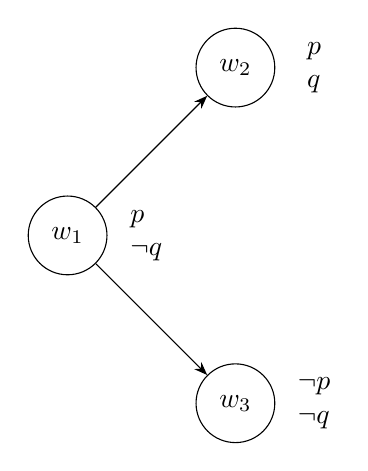
\begin{tikzpicture}[node distance=2cm]

    
    \node[draw, circle, minimum size=1cm, inner sep=2pt, align=center] (w1) {$w_1$};
    \node[draw, circle, minimum size=1cm, inner sep=2pt, align=center] (w2) [above right=of w1] {$w_2$};
    \node[draw, circle, minimum size=1cm, inner sep=2pt, align=center] (w3) [below right=of w1] {$w_3$};

    
    \node[align=left] at ($(w1) + (1,0)$) {$p$\\$\neg q$};
    \node[align=left] at ($(w2) + (1,0)$) {$p$\\$q$};
    \node[align=left] at ($(w3) + (1,0)$) {$\neg p$\\$\neg q$};

    
    \draw[->, >=Stealth] (w1) -- (w2);
    \draw[->, >=Stealth] (w1) -- (w3);

\end{tikzpicture}
}
\end{center}

In this diagram, each circle represents a world, labeled $w_1$, $w_2$, $w_3$, and the propositions that are true in each world are listed next to them. 
The arrows indicate the accessibility relation $R$ between worlds. Formally, when we write $w R w'$, we mean that world $w'$ is accessible from world $w$.

\subsection{Truth at a world}

Every modal model specifies which formulas are true at which worlds.

Let

\[
M = \langle W, R, V \rangle
\]

be a Kripke model over propositional variables $U$. The satisfaction relation

\[
M, w \Vdash \varphi
\]

means ``$\varphi$ is true at world $w$ in $M$.'' It is defined inductively:

\begin{enumerate}
\item Atomic propositions:

    \[
    M, w \Vdash p \leftrightarrow w \in V(p), \quad p \in U
    \]

\item Falsity:

    \[
    M, w \nVdash \bot
    \]

\item Negation:

    \[
    M, w \Vdash \neg \varphi \leftrightarrow M, w \nVdash \varphi
    \]

\item Conjunction:

    \[
    M, w \Vdash \varphi \wedge \psi \leftrightarrow M, w \Vdash \varphi \wedge M, w \Vdash \psi
    \]

\item Disjunction:

    \[
    M, w \Vdash \varphi \vee \psi \leftrightarrow M, w \Vdash \varphi \vee M, w \Vdash \psi
    \]

\item Implication:

    \[
    M, w \Vdash \varphi \to \psi \leftrightarrow M, w \nVdash \varphi \vee M, w \Vdash \psi
    \]

\item Necessity:

    \[
    M, w \Vdash \Box \varphi \leftrightarrow \forall v \in W, (w,w') \in R \to M, w' \Vdash \varphi
    \]

\item Possibility:

    \[
    M, w \Vdash \Diamond \varphi \leftrightarrow \exists w' \in W, (w,w') \in R \wedge M, w' \Vdash \varphi
    \]
\end{enumerate}

\subsection{Truth in a Model}

While

\[
M, w \Vdash \varphi
\]

represents truth at a specific world $w$ (local truth), we sometimes want global truth. Formulas that are true at all worlds in a given model.

\[
M \Vdash \varphi \ \leftrightarrow\ \forall w \in W, \ M, w \Vdash \varphi
\]

That is, $\varphi$ holds at every world in $M$.

\begin{enumerate}
\item If $M \Vdash \varphi$, then $\varphi$ is globally valid in that model.
\item If $M, w \Vdash \varphi$ for some but not all $w$, then $\varphi$ is only locally true in $M$.
\end{enumerate}

\textbf{Example 1:}

Recall the simple model, then we can check which of $p$, $\Box p$, $\Diamond p$, $\Diamond q$ hold and which do not:

\begin{center}
\fbox{
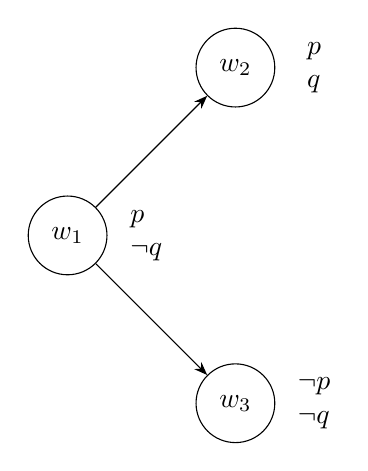
\begin{tikzpicture}[node distance=2cm]

    
    \node[draw, circle, minimum size=1cm, inner sep=2pt, align=center] (w1) {$w_1$};
    \node[draw, circle, minimum size=1cm, inner sep=2pt, align=center] (w2) [above right=of w1] {$w_2$};
    \node[draw, circle, minimum size=1cm, inner sep=2pt, align=center] (w3) [below right=of w1] {$w_3$};

    
    \node[align=left] at ($(w1) + (1,0)$) {$p$\\$\neg q$};
    \node[align=left] at ($(w2) + (1,0)$) {$p$\\$q$};
    \node[align=left] at ($(w3) + (1,0)$) {$\neg p$\\$\neg q$};

    
    \draw[->, >=Stealth] (w1) -- (w2);
    \draw[->, >=Stealth] (w1) -- (w3);

\end{tikzpicture}
}
\end{center}

\begin{enumerate}
\item For $p$:

    \[
    M, w_1 \Vdash p \leftrightarrow w_1 \in V(p)
    \]

    From the model,

    \[
    w_1 \in V(p)
    \]

    Therefore,

    \[
    M, w_1 \Vdash p
    \]

\item For $\Box p$:

    By definition of $\Box$:

    \[
    M, w_1 \Vdash \Box p \leftrightarrow \forall w' \, (w_1 R w' \to M, w' \Vdash p)
    \]

    However:

    \[
    \exists w_3 \, (\, w_1 R w_3 \wedge M, w_3 \nVdash p \,)
    \]

    Consequently, the universal condition fails. Thus,

    \[
    M, w_1 \nVdash \Box p
    \]

\item For $\Diamond p$:

    By definition of $\Diamond$:

    \[
    M, w_1 \Vdash \Diamond p \leftrightarrow \exists w' \, (w_1 R w' \wedge M, w' \Vdash p)
    \]

    From the model,

    \[
    \exists w_2 (w_1 R w_2 \wedge M, w_2 \Vdash p)
    \]

    So the existential condition is satisfied. It follows that,

    \[
    M, w_1 \Vdash \Diamond p
    \]

\item For $\Diamond q$:

    similarly, by definition of $\Diamond$:

    \[
    M, w_1 \Vdash \Diamond q \leftrightarrow \exists w' \, (w_1 R w' \wedge M, w' \Vdash q)
    \]

    From the model,

    \[
    w_1 R w_2 \wedge M, w_2 \Vdash q
    \]

    Thus, the existential condition is satisfied. We conclude that:

    \[
    M, w_1 \Vdash \Diamond q
    \]
\end{enumerate}

\section{Validity and Tautology}

\subsection{Validity}

Validity in modal logic is always a property of formulas. A formula is called valid if it holds in every model and at every world of that model. However, which formulas count as valid depends on the semantics, in particular, on the accessibility relation $R$ that structures the models.

\textbf{Example 1:}

\[
\models \Box(p \land q) \to \Box p
\]

is valid in all Kripke models, since if every accessible world satisfies both $p$ and $q$, then certainly every accessible world satisfies $p$.

\textit{Proof}

Let
\[
M = (W, R, V)
\]

be an arbitrary Kripke model and let

\[
w \in W
\]

be an arbitrary world. We need to show:

\[
M, w \Vdash \Box(p \land q) \to \Box p
\]

First, assume the antecedent

\[
M, w \Vdash \Box(p \land q)
\]

By the semantics of $\Box$, this means:

\[
\forall w' \in W, \text{ if } w R w' \text{ then } M, w' \Vdash p \land q
\]

Second, for each world $w'$ such that $w R w'$:

\[
M, w' \Vdash p \land q \to M, w' \Vdash p
\]


moreover, generalize over accessible worlds.

Since the above holds for all $w'$ accessible from $w$, we have:

\[
\forall w' \in W, \text{ if } w R w' \text{ then } M, w' \Vdash p
\]

By the semantics of $\Box$, this is equivalent to:

\[
M, w \Vdash \Box p
\]

finally, we conclude the implication

\[
M, w \Vdash \Box(p \land q) \to M, w \Vdash \Box p
\]

Ultimatelly,

\[
M, w \Vdash \Box(p \land q) \to \Box p
\]

Since $M$ and $w$ were arbitrary, the formula holds in every world of every Kripke model.

Therefore,

\[
\models \Box(p \land q) \to \Box p. \quad QED
\]

\noindent
\begin{center}
\fbox{
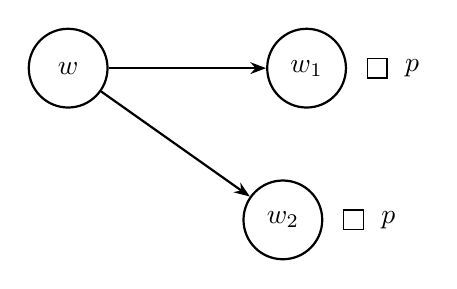
\begin{tikzpicture}[
    node distance=2cm,
    circle node/.style={
        circle,
        draw,
        thick,
        minimum size=1cm,
        inner sep=2pt
    },
    arrow/.style={-{Stealth[length=2mm]}, thick}
]

\node[circle node] (w) {$w$};
\node[circle node, right=of w] (w1) {$w_1$};
\node[circle node, below right=1.2cm and 2cm of w] (w2) {$w_2$};

\draw[arrow] (w) -- (w1);
\draw[arrow] (w) -- (w2);

\node[draw, minimum size=0.25cm, right=0.25cm of w1] (box1) {};
\node[right=0.1cm of box1] {$p$};

\node[draw, minimum size=0.25cm, right=0.25cm of w2] (box2) {};
\node[right=0.1cm of box2] {$p$};

\end{tikzpicture}
}
\end{center}


\textbf{Example 2:}

\[
\Box(p \to q) \not\models p \to \Box q
\]

and

\[
p \to \Box q \not\models \Box(p \to q)
\]

\textit{Proof (by counterexample)}

Let
\[
M = (W,R,V), \quad W = \{w,v\}, \quad R = \{(w,v)\},
\]
with valuation
\[
V(p) = \{w\}, \quad V(q) = \varnothing.
\]


At world $w$:

\begin{enumerate}
\item Antecedent:

\[
M,w \Vdash \Box(p \to q)
\]

because the only accessible world is $v$, and there $p$ is false, so $p \to q$ is true.

\item Consequent:

\[
M,w \not\Vdash p \to \Box q
\]

since $M,w \Vdash p$ but $M,w \not\Vdash \Box q$ (because $q$ is false at $v$).

Therefore,

\[
\Box(p \to q) \not\models p \to \Box q.
\]

\end{enumerate}

\begin{center}
\fbox{
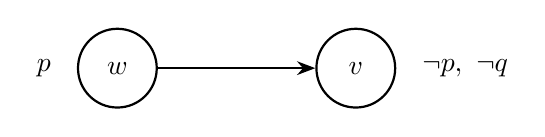
\begin{tikzpicture}[
    node distance=2cm,
    ->,
    >=Stealth,
    thick
]


\tikzstyle{world}=[
    circle,
    draw,
    minimum size=1cm,
    inner sep=2pt,
    align=center
]


\node[world] (w) {$w$};
\node[world, right=of w] (v) {$v$};


\draw (w) -- (v);


\node[left=0.2cm of w] {$p$};
\node[right=0.2cm of v] {$\neg p,\ \neg q$};

\end{tikzpicture}
}
\end{center}

This model makes $\Box(p \to q)$ true at $w$ but $p \to \Box q$ false.

Let

\[
M = (W,R,V), \quad W = \{w,v\}, \quad R = \{(w,v)\},
\]

with valuation

\[
V(p) = \{v\}, \quad V(q) = \varnothing.
\]

At world $w$:

\begin{enumerate}
    \item Antecedent:
    
   \[
    M,w \Vdash p \to \Box q
    \]

    because $M,w \not\Vdash p$, so the implication holds.

    \item consequent:
    
    \[
    M,w \not\Vdash \Box(p \to q)
    \]

    since at $v$, $M,v \Vdash p$ but $M,v \not\Vdash q$, so $p \to q$ is false at $v$.

    Therefore,

   \[
    p \to \Box q \not\models \Box(p \to q). \quad QED
   \]

\end{enumerate}

\begin{center}
\fbox{
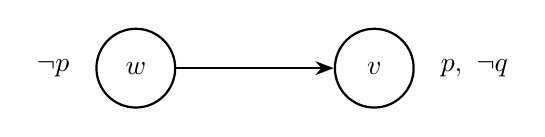
\begin{tikzpicture}[
    node distance=2cm,
    ->,
    >=Stealth,
    thick
]


\tikzstyle{world}=[
    circle,
    draw,
    minimum size=1cm,
    inner sep=2pt,
    align=center
]


\node[world] (w) {$w$};
\node[world, right=of w] (v) {$v$};


\draw (w) -- (v);


\node[left=0.2cm of w] {$\neg p$};
\node[right=0.2cm of v] {$p,\ \neg q$};

\end{tikzpicture}
}
\end{center}


This model makes $p \to \Box q$ true at $w$ but $\Box(p \to q)$ false.

Moreover:

\begin{enumerate}
    \item If $A$ is valid in $U$, then $A$ is valid in every subclass $U' \subseteq U$.
    \item If $A$ is valid, then $\Box A$ is also valid.
\end{enumerate}

\textbf{Example:}

\[
\models \Box X
\]

\textit{Proof}

Assume

\[
\models X
\]

i.e. $X$ is valid in every Kripke model.

Let

\[
M = \langle W, R, V \rangle
\]

be an arbitrary Kripke model and let $w \in W$. Since $X$ is valid, for every world $w' \in W$ we have

\[
M, w' \Vdash X
\]

Now suppose $w R w'$. By validity of $X$, it follows again that

\[
M, w' \Vdash X
\]

Therefore, by the semantics of $\Box$, we obtain

\[
M, w \Vdash \Box X
\]

Since both $M$ and $w$ were arbitrary, we conclude

\[
\models \Box X
\]

\subsection{Tautology}

In classical logic, it is easy to check whether a formula is a tautology or not. For example,

\[P \lor \neg P\]

is a tautology, and we can also prove this using a truth table. However, in modal logic the term tautology is usually not used. 
Instead, we talk about valid formulas, since the semantics of modal logic are more complex than in classical logic. 
In this context, the concept of simultaneous substitution becomes helpful.

For example, recall

\[
\varphi \equiv (\psi \leftrightarrow \chi)
\]

Then under simultaneous substitution we have

\[
\varphi[\delta_1/p_1, \ldots, \delta_n/p_n] \;=\; 
\psi[\delta_1/p_1, \ldots, \delta_n/p_n] \;\leftrightarrow\; 
\chi[\delta_1/p_1, \ldots, \delta_n/p_n].
\]

In other words, substitution distributes structurally through the connectives.

\section{Substitution Lemma}

To justify this notion (e.g. $ \varphi \equiv (\psi \leftrightarrow \chi)$), we prove the Substitution Lemma, which shows that the truth of propositional formulas under an assignment aligns with the truth of their tautological instances in Kripke models.

Suppose $X$ is a modal-free formula whose propositional variables are $x_1, \ldots, x_n$, and let $ \delta_1, \ldots,  \delta_n$ be modal formulas. Then for any assignment $v$, any model $M = \langle W, R, V \rangle$, and any $w \in W$ such that

\[
v(x_i) = T \quad \text{iff} \quad M,w \Vdash \delta_i,
\]

we have

\[
v \Vdash X \quad \text{iff} \quad M,w \Vdash X[ \delta_1/x_1, \ldots,  \delta_n/x_n].
\]

By induction on the structure of $X$.

\begin{enumerate}

\item Atomic variable:

\[
X \equiv x_i
\]

\[
v \Vdash x_i 
\;\leftrightarrow\; v(x_i) = T
\;\leftrightarrow\; M,w \Vdash \delta_i
\;\leftrightarrow\; M,w \Vdash x_i[\delta_1/x_1, \ldots, \delta_n/x_n].
\]

\item Falsity:

\[
X \equiv \bot
\]

\[
v \nVdash \bot 
\quad \text{and} \quad 
M,w \nVdash \bot.
\]

\item Negation:

\[
X \equiv \neg \alpha
\]

\[
v \Vdash \neg \alpha 
\;\leftrightarrow\; v \nVdash \alpha
\;\leftrightarrow\; M,w \nVdash \alpha[\delta_1/x_1, \ldots, \delta_n/x_n]
\;\leftrightarrow\; M,w \Vdash \neg \alpha[\delta_1/x_1, \ldots, \delta_n/x_n].
\]

\item Conjunction:

\[
X \equiv (\alpha \land \beta)
\]

\[
v \Vdash \alpha \land \beta 
\;\leftrightarrow\; (v \Vdash \alpha \land v \Vdash \beta)
\]

\[
\leftrightarrow\; (M,w \Vdash \alpha[\delta_1/x_1, \ldots, \delta_n/x_n]
\land M,w \Vdash \beta[\delta_1/x_1, \ldots, \delta_n/x_n])
\]

\[
\leftrightarrow\; M,w \Vdash (\alpha \land \beta)[\delta_1/x_1, \ldots, \delta_n/x_n].
\]

\item Disjunction:

\[
X \equiv (\alpha \lor \beta)
\]

\[
v \Vdash \alpha \lor \beta 
\;\leftrightarrow\; (v \Vdash \alpha \lor v \Vdash \beta)
\]

\[
\leftrightarrow\; (M,w \Vdash \alpha[\delta_1/x_1, \ldots, \delta_n/x_n]
\lor M,w \Vdash \beta[\delta_1/x_1, \ldots, \delta_n/x_n])
\]

\[
\leftrightarrow\; M,w \Vdash (\alpha \lor \beta)[\delta_1/x_1, \ldots, \delta_n/x_n].
\]

\item Implication:

\[
X \equiv (\alpha \to \beta)
\]

\[
v \Vdash \alpha \to \beta 
\;\leftrightarrow\; (v \nVdash \alpha \lor v \Vdash \beta)
\]

\[
\leftrightarrow\; (M,w \nVdash \alpha[\delta_1/x_1, \ldots, \delta_n/x_n]
\lor M,w \Vdash \beta[\delta_1/x_1, \ldots, \delta_n/x_n])
\]

\[
\leftrightarrow\; M,w \Vdash (\alpha \to \beta)[\delta_1/x_1, \ldots, \delta_n/x_n].
\]

\end{enumerate}

From this lemma we can show that all tautological instances are valid. Contrapositively, suppose $U$ is such that

\[
M,w \nVdash U[ \delta_1/x_1,\ldots, \delta_n/x_n]
\]

for some model $M$ and world $w$. Define an assignment $v$ such that

\[
v(x_i) = T \quad \leftrightarrow \quad M,w \Vdash \delta_i,
\]

and let $v$ assign arbitrary values to $q \notin \{x_1, \ldots, x_n\}$. Then by the lemma,  

\[
v \Vdash U,
\]

so $U$ is not a tautology.

\section{Schema}

A schema is a collection of formulas consisting precisely of all substitution instances of a given modal formula $\varphi$. Formally:

\[
\{ \psi : \exists \delta_1, \ldots, \delta_n\; (\psi = \varphi[\delta_1/x_1, \ldots,\delta_n/x_n]) \}
\]

The formula $\varphi$ is called the characteristic formula of the schema, and it is unique up to renaming of propositional variables. A formula $\psi$ is said to be an instance of a schema if $\psi$ belongs to this set.

For convenience, a schema is usually denoted by a meta-linguistic expression obtained by substituting symbols such as $A, B, \dots$ for propositional variables. For example:

\begin{enumerate}

\item The schema $A$ corresponds to the characteristic formula $p$.

\item The schema $A \to \Box A$ corresponds to $p \to \Box p$.

\item The schema $A \to (B \to A)$ corresponds to $p \to (q \to p)$.

\end{enumerate}

In particular, the schema $A$ denotes the set of all formulas, since every formula is a substitution instance of $p$.

\subsection{Truth and Validity}

A schema is said to be true in a model if and only if all of its instances are true in that model. Similarly, a schema is valid if and only if it is true in every model. Valid schemas have a particularly important connection with the axiom schema $K$:

$$K = \Box(A \to B) \to (\Box A \to \Box B).$$

It can be shown that $K$ is valid in every model. Because of this, schema $K$ serves as the cornerstone of the modal system $K$, the weakest normal modal logic.


\subsection{Valid Schemas}

The following schemas are valid in every Kripke model:

\begin{enumerate}

\item $\Box(A \to B) \to (\Diamond A \to \Diamond B)$

\item $\Diamond(A \to B) \to (\Box A \to \Diamond B)$

\item $\Box(A \land B) \leftrightarrow (\Box A \land \Box B)$

\item $\Box A \to \Box(B \to A)$

\item $\neg \Diamond A \to \Box(A \to B)$

\item $\Diamond(A \lor B) \leftrightarrow (\Diamond A \lor \Diamond B)$

\item $\Diamond A \leftrightarrow \neg \Box \neg A$

\end{enumerate}

\textbf{Example:}

Let $M = (W, R, V)$ be an arbitrary Kripke model and $w \in W$ an arbitrary world.
We show the duality of $\Diamond$ and $\Box$:

\begin{enumerate}

\item By definition:

\[
M, w \Vdash \neg \Box \neg A \leftrightarrow M, w \nVdash \Box \neg A.
\]

\item By the semantics of $\Box$:

\[
M, w \Vdash \Box \neg A 
\leftrightarrow \forall w' \in W,\,(w R w' \to M, w' \Vdash \neg A).
\]

Therefore:

\[
M, w \nVdash \Box \neg A 
\leftrightarrow \neg(\forall w' \in W,\,(w R w' \to M, w' \Vdash \neg A)).
\]

\item Negating the universal gives an existential:

\[
\neg(\forall w' \in W,\,(w R w' \to M, w' \Vdash \neg A))
\leftrightarrow \exists w' \in W,\,(w R w' \wedge M, w' \nVdash \neg A).
\]

\item By classical negation:

\[
M, w' \nVdash \neg A \leftrightarrow M, w' \Vdash A.
\]

\item By definition of $\Diamond$:

\[
\exists w' \in W,\,(w R w' \wedge M, w' \Vdash A)
\leftrightarrow M, w \Vdash \Diamond A.
\]

\end{enumerate}

Thus, for an arbitrary model $M$ and world $w$:

\[
M, w \Vdash \Diamond A \leftrightarrow M, w \Vdash \neg \Box \neg A.
\]

Since $M$ and $w$ were arbitrary, the formula is valid in all Kripke models:

\[
\models \Diamond A \leftrightarrow \neg \Box \neg A.
\]

\subsection{Invalid Schemas}

To show that a formula $\varphi$ is invalid, we construct a model $M$ and a world $w$ such that  

\[M, w \not\Vdash \varphi\]

Such models are called falsifying models. To show that a schema $X$ is invalid, it suffices to construct a falsifying model for one of its instances.

\textbf{Example 1:}

Schema $D$ is

\[
\Box p \to \Diamond p.
\]

Counterexample:

Let

\[
M = (W, R, V)
\]

with

\[
W = \{w\}, \quad R = \varnothing, \quad V(p) = \varnothing.
\]

\begin{enumerate}

\item Antecedent:

\[
M, w \Vdash \Box p
\leftrightarrow \forall v \in W\,(w R v \Rightarrow M, v \Vdash p).
\]

Since $R = \varnothing$,

\[
M, w \Vdash \Box p.
\]

\item Consequent:

\[
M, w \Vdash \Diamond p
\leftrightarrow \exists v \in W\,(w R v \land M, v \Vdash p).
\]

Since $R = \varnothing$,

\[
M, w \nVdash \Diamond p.
\]

\item Therefore:

\[
M, w \nVdash \Box p \to \Diamond p.
\]

\end{enumerate}

Hence $\Box p \to \Diamond p$ is not valid. \quad Q.E.D.



\begin{center}
\fbox{
\begin{tikzpicture}[
    node distance=2cm,
    ->,
    >=Stealth,
    thick
]

\tikzstyle{world}=[
    circle,
    draw,
    minimum size=1cm,
    inner sep=2pt,
    align=center
]


\node[world, label=below:$\neg p$] (w) at (0,0) {$w$};

\node[world] (w1) at (-3,0) {$w_1$};
\node[world] (w2) at (3,0) {$w_2$};
\node[world] (w3) at (0,3) {$w_3$};
\node[world] (w4) at (0,-3) {$w_4$};

\node[below=0.5cm of w] {$M, w \not\Vdash \Box p \to \Diamond p$};

\end{tikzpicture}
}
\end{center}

\textbf{Example 2:}

Schema $T$ is

\[
\Box p \to p.
\]

Counterexample:

Let

\[
M = (W, R, V)
\]

with

\[
W = \{w\}, \quad R = \varnothing, \quad V(p) = \varnothing.
\]

\begin{enumerate}

\item Antecedent:

\[
M, w \Vdash \Box p
\leftrightarrow \forall v \in W\,(w R v \Rightarrow M, v \Vdash p).
\]

Since $R = \varnothing$,

\[
M, w \Vdash \Box p.
\]

\item Consequent:

\[
M, w \Vdash p
\]

is false because $V(p) = \varnothing$. Hence,

\[
M, w \nVdash p.
\]

\item Therefore:

\[
M, w \nVdash \Box p \to p.
\]

\end{enumerate}

Hence $\Box p \to p$ is not valid. \quad Q.E.D.

\begin{center}
\fbox{
\begin{tikzpicture}[
    node distance=2cm,
    ->,
    >=Stealth,
    thick
]

\tikzstyle{world}=[
    circle,
    draw,
    minimum size=1cm,
    inner sep=2pt,
    align=center
]


\node[world, label=below:$\neg p$] (w) at (0,0) {$w$};


\node[world] (w1) at (-3,0) {$w_1$};
\node[world] (w2) at (3,0) {$w_2$};
\node[world] (w3) at (0,3) {$w_3$};
\node[world] (w4) at (0,-3) {$w_4$};



\node[below=0.5cm of w] {$M, w \not\Vdash \Box p \to p$};

\end{tikzpicture}
}
\end{center}

\textbf{Example 3:}

Schema $B$ is:

\[
p \to \Box\Diamond p.
\]

Counterexample:

Let

\[
M = (W, R, V)
\]

with

\[
W = \{w, v\}, \quad R = \{(w, v)\}, \quad V(p) = \{w\}.
\]

\begin{enumerate}

\item Antecedent:

\[
M, w \Vdash p
\]

since $w \in V(p)$.

\item Consequent:

\[
M, w \Vdash \Box\Diamond p
\leftrightarrow \forall x \in W\,(w R x \Rightarrow M, x \Vdash \Diamond p).
\]

There is $x = v$ with $w R v$. But

\[
M, v \Vdash \Diamond p
\leftrightarrow \exists u \in W\,(v R u \land M, u \Vdash p),
\]

and there is no $u$ with $v R u$. Hence,

\[
M, v \nVdash \Diamond p,
\]
so

\[
M, w \nVdash \Box\Diamond p.
\]

\item Therefore:

\[
M, w \nVdash p \to \Box\Diamond p.
\]

\end{enumerate}

Hence $p \to \Box\Diamond p$ is not valid. \quad Q.E.D.

\begin{center}
\fbox{
\begin{tikzpicture}[
    ->,
    >=Stealth,
    thick,
    node distance=2cm
]

\tikzstyle{world}=[
    circle,
    draw,
    minimum size=1cm,
    inner sep=2pt,
    align=center
]


\node[world, label=below:$p$] (w) at (0,0) {$w$};
\node[world, label=below:$\neg p$] (v) at (3,0) {$v$};


\node[world] (w1) at (-3,0) {$w_1$};
\node[world] (w2) at (0,3) {$w_2$};
\node[world] (w3) at (0,-3) {$w_3$};


\draw (w) -- (v);

\node[below=0.5cm of w] {$M, w \not\Vdash p \to \Box\Diamond p$};

\end{tikzpicture}
}
\end{center}

\textbf{Example 4:}

Schema \textbf{4} is

\[
\Box p \to \Box\Box p.
\]

Counterexample:

Let

\[
M = (W, R, V)
\]

with

\[
W = \{w, v, u\}, \quad R = \{(w, v), (v, u)\}, \quad V(p) = \{v\}.
\]

\begin{enumerate}

\item Antecedent:

\[
M, w \Vdash \Box p
\leftrightarrow \forall x \in W\,(w R x \Rightarrow M, x \Vdash p).
\]

The only $x$ with $w R x$ is $v$, and $v \in V(p)$, so

\[
M, w \Vdash \Box p.
\]

\item Consequent:

\[
M, w \Vdash \Box\Box p
\leftrightarrow \forall x \in W\,(w R x \Rightarrow M, x \Vdash \Box p).
\]

For $x = v$ we have

\[
M, v \Vdash \Box p
\leftrightarrow \forall y \in W\,(v R y \Rightarrow M, y \Vdash p).
\]

But $v R u$ and $u \notin V(p)$, hence

\[
M, v \nVdash \Box p,
\]

so

\[
M, w \nVdash \Box\Box p.
\]

\item Therefore:

\[
M, w \nVdash \Box p \to \Box\Box p.
\]

\end{enumerate}

Hence $\Box p \to \Box\Box p$ is not valid. \quad Q.E.D.

\begin{center}
\fbox{
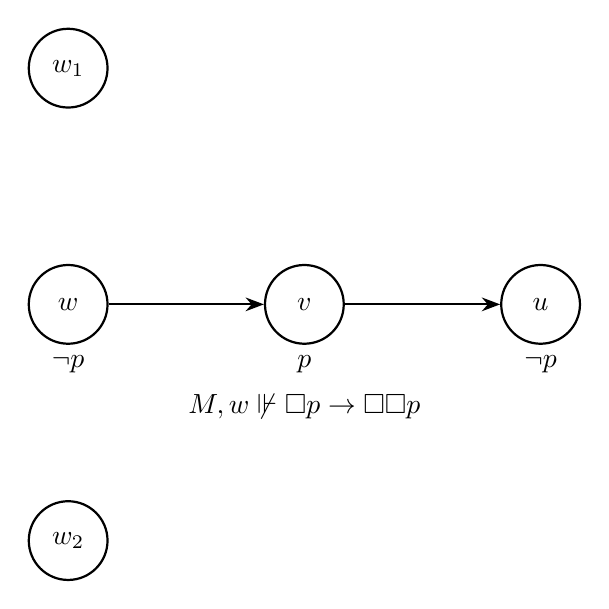
\begin{tikzpicture}[
    ->,
    >=Stealth,
    thick,
    node distance=2cm
]

\tikzstyle{world}=[
    circle,
    draw,
    minimum size=1cm,
    inner sep=2pt,
    align=center
]


\node[world, label=below:$\neg p$] (w) at (0,0) {$w$};
\node[world, label=below:$p$] (v) at (3,0) {$v$};
\node[world, label=below:$\neg p$] (u) at (6,0) {$u$};


\node[world] (w1) at (0,3) {$w_1$};
\node[world] (w2) at (0,-3) {$w_2$};

\draw (w) -- (v);
\draw (v) -- (u);


\node[below=0.5cm of v] {$M, w \not\Vdash \Box p \to \Box\Box p$};

\end{tikzpicture}
}
\end{center}

\textbf{Example 5:}

Schema \textbf{5} is

\[
\Diamond p \to \Box\Diamond p.
\]

Counterexample:

Let

\[
M = (W, R, V)
\]

with

\[
W = \{w, v\}, \quad R = \{(w, v)\}, \quad V(p) = \{v\}.
\]

\begin{enumerate}

\item Antecedent:

\[
M, w \Vdash \Diamond p
\leftrightarrow \exists x \in W\,(w R x \land M, x \Vdash p).
\]

Since $w R v$ and $v \in V(p)$,

\[
M, w \Vdash \Diamond p.
\]

\item Consequent:

\[
M, w \Vdash \Box\Diamond p
\leftrightarrow \forall x \in W\,(w R x \Rightarrow M, x \Vdash \Diamond p).
\]

The only $x$ with $w R x$ is $v$, and

\[
M, v \Vdash \Diamond p
\leftrightarrow \exists y \in W\,(v R y \land M, y \Vdash p).
\]

There is no $y$ with $v R y$, hence

\[
M, v \nVdash \Diamond p,
\]

so

\[
M, w \nVdash \Box\Diamond p.
\]

\item Therefore:

\[
M, w \nVdash \Diamond p \to \Box\Diamond p.
\]

\end{enumerate}

Hence $\Diamond p \to \Box\Diamond p$ is not valid. \quad Q.E.D.

\begin{center}
\fbox{
\begin{tikzpicture}[
    ->,
    >=Stealth,
    thick,
    node distance=2cm
]

\tikzstyle{world}=[
    circle,
    draw,
    minimum size=1cm,
    inner sep=2pt,
    align=center
]


\node[world, label=below:$\neg p$] (w) at (0,0) {$w$};
\node[world, label=below:$p$] (v) at (3,0) {$v$};


\node[world] (w1) at (-3,0) {$w_1$};
\node[world] (w2) at (0,3) {$w_2$};
\node[world] (w3) at (0,-3) {$w_3$};


\draw (w) -- (v);

\node[below=0.5cm of w] {$M, w \not\Vdash \Diamond p \to \Box\Diamond p$};

\end{tikzpicture}
}
\end{center}

\subsection{Properties of Schemas}

If $A$ and $A \to B$ are true at a world $w$ in a model $M$, then $B$ must also be true at $w$. 
This follows immediately from the semantics of implication. Hence, the class of valid formulas is closed under modus ponens. 
A formula $A$ is valid if and only if all its substitution instances are valid. Equivalently, a schema is valid if and only if its characteristic formula is valid. The “if” direction is straightforward: 
$A$ is trivially a substitution instance of itself, so if $A$ is valid, then one substitution instance (namely $A$ itself) is valid. For the “only if” direction, suppose $M = \langle W,R,V\rangle$ is a modal model, and let  

\[
B \equiv A[D_1/p_1, \ldots, D_n/p_n]
\]

be a substitution instance of $A$. Construct a new model $M' = \langle W,R,V'\rangle$ where

\[ V'(p_i) = \{w \in W : M,w \Vdash D_i\}.\]

One proves by induction on the structure of $A$ that, for all $w \in W$,

\[
M,w \Vdash B \quad \text{iff} \quad M',w \Vdash A.
\]

If $A$ were valid but some substitution instance $B$ were not valid, then there would exist $M,w$ such that $M,w \not\Vdash B$. 
By the equivalence above, this would imply $M',w \not\Vdash A$, contradicting the assumption that $A$ is valid.
Thus, every substitution instance of $A$ must also be valid. By contrast, truth in a particular model does not behave in the same way. 

For example, let $A = p$ in a model with a single world $w$ and valuation $V(p) = \{w\}$. 
Then $p$ is true at $w$. However, $\bot$ is also a substitution instance of $p$, yet $\bot$ is not true at $w$. 
Thus, while validity is preserved under substitution, truth in a specific model is not.

\section{Frame Definability}

A frame is a pair $F = \langle W, R \rangle$ where $W$ is a non-empty set of worlds
and $R$ is a binary relation on $W$. A model $M$ is based on a frame
$F = \langle W, R \rangle$ iff $M = \langle W, R, V \rangle$ for some valuation $V$.
We say that a formula $A$ is valid in a frame $F$, written $F \vDash A$, if
$M \vDash A$ for every model $M$ based on $F$.

More generally, if $\mathcal{F}$ is a class of frames, then $A$ is valid in
$\mathcal{F}$, written $\mathcal{F} \vDash A$, iff $F \vDash A$ for every frame
$F \in \mathcal{F}$. If $\mathcal{F}$ is a class of frames, we say that $A$
\emph{defines} $\mathcal{F}$ iff $\mathcal{F} \vDash A$ for all and only frames
$F \in \mathcal{F}$.

While a model $M$ may guarantee the truth of a formula, this can occur only because
of a particular valuation $V$. In such cases, the truth is merely an
\emph{accidental truth}: it holds due to how truth values were assigned, not
because of the frame’s structure. A frame, on the other hand, concerns only the
behavior and relationships of worlds, not the propositional variables themselves.
Thus, if a formula is valid on a frame, it reflects a genuine structural property
of that frame rather than a coincidental choice of valuation.

\textbf{Example:}

\begin{enumerate}
  \item Reflexive frame:
  
  \[
  \forall w \in W,\; w R w
  \]

  Therefore:

  \[
  M, w \Vdash \Box A \rightarrow A \quad \text{for all } M \text{ on } F
  \]

  \item Accidental truth in a non-reflexive model:
  
  \[
  F = \langle \{w\}, \varnothing \rangle
  \]

  \[
  M = \langle \{w\}, \varnothing, V \rangle \quad \text{with } V(p) = \{w\}
  \]

  Then:

  \[
  M, w \Vdash \Box p \rightarrow p
  \]

  \item Non-reflexive frame:
  
  \[
  \exists w \in W,\; \neg w R w
  \]

  where:

  \[
  V(p) = W \setminus \{w\}
  \]

  Then:

  \[
  M, w \not\Vdash \Box p \rightarrow p
  \]
\end{enumerate}

As we can see from the example, a frame $F$ is simply a pair

\[
F = \langle W, R \rangle
\]  

consisting of a set of worlds $W$ with an accessibility relation $R$.  

Every model

\[
M = \langle W, R, V \rangle
\]

is then, as we say, based on the frame $\langle W, R \rangle$.  


We can now define $F \Vdash A$, the notion of a formula being *valid in a frame*, as:  

\[
M \Vdash A \quad \text{for all } M \text{ based on } F
\]  

With this notation, we can establish correspondence relations between formulas and classes of frames.  

For example:  

\[F \Vdash \Box p \rightarrow p \quad \text{iff} \quad F \text{ is reflexive.}\]

\subsection{Properties of Accessibility Relations}

Recall that in Invalid Schemas we constructed counterexamples showing that the schemas $(D, T, B, 4, 5)$ are not valid in general Kripke frames. In this part, we will prove that these schemas are indeed valid whenever the accessibility relation $R$ has the corresponding property.  

Let

\[
M = \langle W, R, V \rangle
\]

be a Kripke model. If $R$ has one of the properties (serial, reflexive, symmetric, transitive, euclidean), then the corresponding modal axiom

\[
(D, T, B, 4, 5) \text{ is valid in } M.
\]


\begin{enumerate}
    \item Serial ($D$)

    Let

    \[
    M = (W, R, V)
    \]

    be an arbitrary Kripke model with $R$ serial.

    Let
    \[
    w \in W
    \]

    be an arbitrary world. We need to show

    \[
    M, w \Vdash \Box p \to \Diamond p
    \]

    First, assume

    \[
    M, w \Vdash \Box p
    \]

    by definition of $\Box$,

    \[
    \forall v \in W\; (w R v \to M, v \Vdash p)
    \]

    Second, since $R$ is serial

    \[
    \exists v \in W \; (w R v)
    \]

    From the assumption

    \[
    M, v \Vdash p
    \]

    Third

    \[
    \exists v \in W \; (w R v \land M, v \Vdash p)
    \]

    Thus

    \[
    M, w \Vdash \Diamond p
    \]

    Finally

    \[
    M, w \Vdash \Box p \to \Diamond p
    \]

    We conclude that

    \[
    \models \Box p \to \Diamond p \quad Q.E.D.
    \]

    \item Reflexive ($T$)
    
    Let

    \[
    M = (W, R, V)
    \]

    be an arbitrary Kripke model with $R$ reflexive.

    Let

    \[
    w \in W
    \]

    be an arbitrary world. We need to show

    \[
    M, w \Vdash \Box p \to p
    \]

    First, assume

    \[
    M, w \Vdash \Box p
    \]

    By definition of $\Box$,

    \[
    \forall v \in W\; (w R v \to M, v \Vdash p)
    \]

    Second, since $R$ is reflexive

    \[
    w R w
    \]

    From the assumption

    \[
    M, w \Vdash p
    \]

    Finally

    \[
    M, w \Vdash \Box p \to p
    \]

    As a consequence

    \[
    \models \Box p \to p \quad Q.E.D.
    \]

    \item Symmetric ($B$)
    
    Let

    \[
    M = (W, R, V)
    \]

    be an arbitrary Kripke model with $R$ symmetric.

    Let
    \[
    w \in W
    \]

    be an arbitrary world. We need to show

    \[
    M, w \Vdash p \to \Box \Diamond p
    \]

    First, assume

    \[
    M, w \Vdash p
    \]

    Second, let $v \in W$ with

    \[
    w R v
    \]

    Since $R$ is symmetric

    \[
    v R w
    \]

    Third, from the assumption

    \[
    M, w \Vdash p
    \]

    we obtain

    \[
    M, v \Vdash \Diamond p
    \]

    Finally

    \[
    M, w \Vdash \Box \Diamond p
    \]

    As a result

    \[
    \models p \to \Box \Diamond p \quad Q.E.D.
    \]

    \item Transitive ($4$)
    
    Let

    \[
    M = (W, R, V)
    \]

    be an arbitrary Kripke model with $R$ transitive. 

    Let
    \[
    w \in W
    \]

    be an arbitrary world. We need to show

    \[
    M, w \Vdash \Box p \to \Box \Box p
    \]

    First, assume

    \[
    M, w \Vdash \Box p
    \]

    By definition of $\Box$,

    \[
    \forall v \in W\; (w R v \to M, v \Vdash p)
    \]

    Second, take an arbitrary $v \in W$ such that

    \[
    w R v
    \]

    From the assumption,

    \[
    M, v \Vdash p
    \]

    And for all $u \in W$ with

    \[
    v R u
    \]

    Since $R$ is transitive,

    \[
    w R u
    \]

    Thus from the assumption,

    \[
    M, u \Vdash p
    \]

    Therefore

    \[
    M, v \Vdash \Box p
    \]

    Finally

    \[
    M, w \Vdash \Box \Box p
    \]

    Consequently

    \[
    \models \Box p \to \Box \Box p \quad Q.E.D.
    \]

    \item Euclidean ($5$)
    
    Let

    \[
    M = (W, R, V)
    \]

    be an arbitrary Kripke model with $R$ euclidean. 

    Let

    \[
    w \in W
    \]
    
    be an arbitrary world. We need to show

    \[
    M, w \Vdash \Diamond p \to \Box \Diamond p
    \]

    First, assume

    \[
    M, w \Vdash \Diamond p
    \]

    By definition of $\Diamond$,

    \[
    \exists v \in W \; (w R v \land M, v \Vdash p)
    \]

    Second, take an arbitrary $u \in W$ such that

    \[
    w R u
    \]

    Since $R$ is euclidean and $w R v$,

    \[
    u R v
    \]

    Third, from

    \[
    M, v \Vdash p
    \]

    we obtain

    \[
    M, u \Vdash \Diamond p
    \]

    Finally

    \[
    M, w \Vdash \Box \Diamond p
    \]

    It follows that

    \[
    \models \Diamond p \to \Box \Diamond p \quad Q.E.D.
    \]

\end{enumerate}

\subsection{Partially Functional Relation}

A relation $R$ on a set of worlds $W$ is partially functional if  

\[
\forall w \in W, \; \forall u,v \in W, \; (w R u \wedge w R v \to u = v)
\]

This means each world has at most one accessible world.

\textbf{Example:}

Let

\[
M = (W,R,V), \quad W = \{w,v\}, \quad R = \{(w,v)\}.
\]

Since from $w$ there is at most one successor, we have

\[
wRv \;\;\text{and no other $R$-successor of $w$}.
\]

Therefore, the partial functionality condition holds:

\[
\forall x \in W,\; \forall y,z \in W,\; (xRy \wedge xRz) \;\to\; y = z.
\]

Therefore,
  
\[
R \text{ is partially functional.}
\]

\subsection{Functional Relation}

A relation $R$ on a set of worlds $W$ is functional if  

$$
\forall w \in W, \; \exists v \in W \, \big(w R v \;\wedge\; \forall u \in W, (w R u \to u = v)\big)
$$

This ensures exactly one accessible world per world.

\textbf{Example:}

Let  

\[
M = (W,R,V), \quad W = \{w,v,u\}, \quad R = \{(w,v), (v,u), (u,w)\}.
\]

Since from each world there is exactly one successor, we have  

\[
(wRv) \wedge (vRu) \wedge (uRw).
\]

Therefore, the functionality condition holds:  

\[
\forall x \in W,\; \exists! y \in W \;\; (xRy).
\]

Thus,

\[
R \text{ is functional.}
\]

\begin{center}
\fbox{
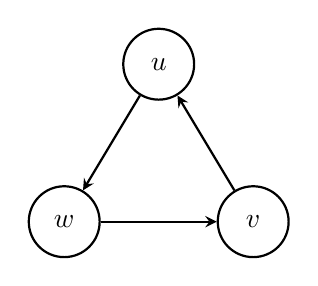
\begin{tikzpicture}[->,>=stealth,thick,node distance=2cm]
  \tikzstyle{world}=[circle,draw,minimum size=0.9cm,align=center]

  \node[world] (w) at (0,0) {$w$};
  \node[world] (v) at (2.4,0) {$v$};
  \node[world] (u) at (1.2,2) {$u$};

  \draw (w) -- (v);
  \draw (v) -- (u);
  \draw (u) -- (w);

\end{tikzpicture}
}
\end{center}


\subsection{Weakly Dense Relation}

A relation $R$ is weakly dense if whenever $uRv$, there is a $w$ ``between" $u$ and $v$.

$$
\forall u,v \in W, \; (u R v \to \exists w \in W \; (u R w \wedge w R v))
$$

\textbf{Example:}

Let  

\[
M = (W,R,V), \quad W = \{w,u,v\}, \quad R = \{(w,u), (u,v), (w,v)\}.
\]

Since there is a direct relation $wRv$, and also an intermediate path through $u$, we have  

\[
\exists w,u,v \in W \;\; (wRv \wedge wRu \wedge uRv).
\]

Therefore, the weak density condition holds:  

\[
\forall w,v \in W,\; (wRv) \;\to\; \exists u \in W \;(wRu \wedge uRv).
\]

Accordingly,

\[
R \text{ is weakly dense.}
\]

\begin{center}
\fbox{
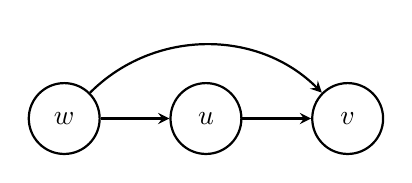
\begin{tikzpicture}[->,>=stealth,thick,node distance=1.8cm]
  \tikzstyle{world}=[circle,draw,minimum size=0.9cm,align=center]

  \node[world] (w) at (0,0) {$w$};
  \node[world] (u) at (1.8,0) {$u$};
  \node[world] (v) at (3.6,0) {$v$};

  \draw (w) -- (u);
  \draw (u) -- (v);
  \draw[bend left=45] (w) to (v);

\end{tikzpicture}
}
\end{center}

\subsection{Confluence (Diamond Property)}

A relation $R$ on $W$ is confluent if  

$$
\forall w,u,v \in W, \; (w R u \wedge w R v) \to \exists t \in W \; (u R t \wedge v R t)
$$  

\textbf{Example:}

Let

\[
M = (W,R,V), \quad W = \{w,u,v,t\}, \quad R = \{(w,u),(w,v),(u,t),(v,t)\}.
\]

Since from $w$ we can reach both $u$ and $v$, we have

\[
\exists w,u,v,t \in W \;\; (wRu \wedge wRv \wedge uRt \wedge vRt).
\]

Therefore, the confluence condition holds:  

\[
\forall w,u,v \in W,\; (wRu \wedge wRv) \;\to\; \exists t \in W \;(uRt \wedge vRt).
\]

Because of this,

\[
R \text{ is confluent.}
\]

\begin{center}
\fbox{
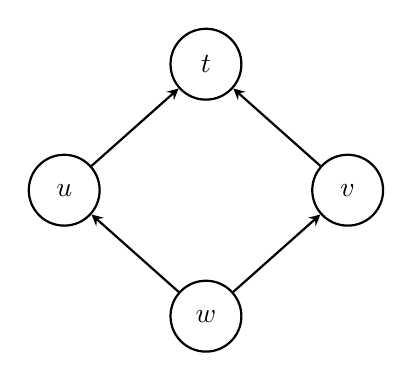
\begin{tikzpicture}[->,>=stealth,thick,node distance=2cm]
  \tikzstyle{world}=[circle,draw,minimum size=0.9cm,align=center]

  
  \node[world] (w) at (0,0) {$w$};
  \node[world] (u) at (-1.8,1.6) {$u$};
  \node[world] (v) at (1.8,1.6) {$v$};
  \node[world] (t) at (0,3.2) {$t$};

  
  \draw (w) -- (u);
  \draw (w) -- (v);
  \draw (u) -- (t);
  \draw (v) -- (t);

\end{tikzpicture}
}
\end{center}

\section{Combining Frame Properties}

\begin{enumerate}

\item $T + 4 = S4$

Suppose

\[
M = (W, R, V), \quad W = \{w, v, u\}
\]

with the relation

\[
R = \{(w,w), (v,v), (u,u), (w,v), (v,u), (w,u)\}.
\]

Reflexivity ($T$):

\[
\forall x \in W \; (xRx)
\]

Holds, since \( wRw, vRv, uRu \in R \).

Transitivity ($4$):

\[
\forall x,y,z \in W \; (xRy \wedge yRz \to xRz)
\]

Holds, since \( wRv \wedge vRu \to wRu \in R \).

Modal validity at $w$:

\[
M,w \Vdash \Box p \to p
\]

\[
M,w \Vdash \Box p \to \Box \Box p
\]

It follows that $R$ is reflexive and transitive, validating $S4$.

\item $T + B$

Suppose

\[
M = (W, R, V), \quad W = \{w, v, u\}
\]

with the relation

\[
R = \{(w,w), (v,v), (u,u), (w,v), (v,w)\}.
\]

Reflexivity ($T$):

\[
\forall x \in W \; (xRx)
\]

Symmetry ($B$):

\[
\forall x,y \in W \; (xRy \to yRx)
\]

Modal validity at $w$:

\[
M,w \Vdash \Box p \to p
\]

\[
M,w \Vdash p \to \Box \Diamond p
\]

As a result $R$ is reflexive and symmetric.

\item $T + 5 = S5$

Suppose

\[
M = (W, R, V), \quad W = \{w, v, u\}
\]

with

\[
R = W \times W.
\]

Reflexivity ($T$):

\[
\forall x \in W \; (xRx)
\]

Euclidean ($5$):

\[
\forall x,y,z \in W \; (xRy \wedge xRz \to yRz)
\]

Modal validity at $w$:

\[
M,w \Vdash \Box p \to p
\]

\[
M,w \Vdash \Diamond p \to \Box \Diamond p
\]

Thus, $R$ is reflexive and Euclidean, validating $S5$.

\item $B + 5$

Suppose

\[
M = (W, R, V), \quad W = \{w, v, u\}
\]

with the relation

\[
R = \{(w,w), (v,v), (u,u), (w,v), (v,w), (v,u), (u,v)\}.
\]

Symmetry ($B$):

\[
\forall x,y \in W \; (xRy \to yRx)
\]

Euclidean ($5$):

\[
\forall x,y,z \in W \; (xRy \wedge xRz \to yRz)
\]

Modal validity at $w$:

\[
M,w \Vdash p \to \Box \Diamond p
\]

\[
M,w \Vdash \Diamond p \to \Box \Diamond p
\]

Accordingly $R$ is symmetric and Euclidean.

\item $4 + 5$

Suppose

\[
M = (W, R, V), \quad W = \{w, v, u\}
\]

with the relation

\[
R = \{(w,w), (v,v), (u,u), (w,v), (v,u), (w,u)\}.
\]

Transitivity ($4$):

\[
\forall x,y,z \in W \; (xRy \wedge yRz \to xRz)
\]

Euclidean ($5$):

\[
\forall x,y,z \in W \; (xRy \wedge xRz \to yRz)
\]

Modal validity at $w$:

\[
M,w \Vdash \Box p \to \Box \Box p
\]

\[
M,w \Vdash \Diamond p \to \Box \Diamond p
\]

We conclude that $R$ is transitive and Euclidean.

\end{enumerate}

\section{Logical Relationships Between Properties}

\begin{enumerate}

\item $T \to D$

\emph{Proof.}

Assume $R$ is reflexive:

\[
\forall w \in W: wRw
\]

We show $R$ is serial:

\[
\forall w \in W \mid \exists v \in W: wRv
\]

Let $w \in W$. By reflexivity, $wRw$, so choose $v = w$.

As a consequence $R$ is serial. $QED$

\item $B + 4 \to 5$

\emph{Proof.}

Assume symmetry and transitivity:

\[
\forall x,y: xRy \to yRx
\]

\[
\forall x,y,z \mid (xRy \land yRz) \to xRz
\]

Let \[xRy \land xRz\] 

By symmetry, \[yRx\]

By transitivity, \[yRx \land xRz \to yRz\]

Thererfore $R$ is Euclidean. $QED$

\item $T + 5 \to B$

\emph{Proof.}

Assume reflexivity and Euclideanness.

Let \[xRy\] 

By reflexivity, \[xRx\]

By Euclidean property:

\[
(xRy \land xRx) \to yRx
\]

Thus $R$ is symmetric. $QED$

\item $B + 5 \to 4$

\emph{Proof.}

Assume symmetry and Euclideanness.

Let 

\[xRy \land yRz\]

By symmetry, \[yRx\]

By Euclidean property:

\[
(yRx \land yRz) \to xRz
\]

Hence $R$ is transitive. $QED$

\item $D + B + 4 \to T$

\emph{Proof}

Assume seriality, symmetry, and transitivity.

Let \[w \in W\]

By seriality, \[\exists v \mid wRv\]

By symmetry, \[vRw\]

By transitivity:

\[
(wRv \land vRw) \to wRw
\]

Thus $R$ is reflexive. $QED$

\end{enumerate}

\section{Frame Definability in FOL and SOL}

We have seen that a number of properties of accessibility relations of frames can be defined by modal formulas. For instance, symmetry of frames can be defined by the formula:

\[
B: \quad p \to \Box \Diamond p
\]

The conditions encountered so far can all be expressed by first-order formulas in a language involving a single two-place predicate symbol \(Q\). For example:

\[
\forall x \forall y \,(Q(x,y) \to Q(y,x))
\]

A first-order structure \(M\) with \(|M| = W\) and \(Q^M = R\) satisfies this formula if and only if \(R\) is symmetric.

\subsection{First-Order Definability}

A class \(\mathcal{F}\) of frames is \emph{FO-definable} if there exists a first-order sentence \(A\) with a single two-place predicate \(Q\) such that for all frames \(F = \langle W, R \rangle\):

\[
F \in \mathcal{F} \leftrightarrow M \models A,
\]
where \(|M| = W\) and \(Q^M = R\).

\textbf{Example:}

Take the FO sentence:

\[
A := \forall x \forall y \,(Q(x,y) \to Q(y,x)).
\]

Let \(\mathcal{F}\) be the class of all symmetric frames. If

\[
F = \langle W,R \rangle,
\quad
W = \{w_1, w_2\},
\quad
R = \{(w_1,w_2),(w_2,w_1),(w_1,w_1),(w_2,w_2)\},
\]

then the associated structure \(M\) satisfies \(A\). If \(R\) is not symmetric, then \(M \not\models A\). Hence, \(\mathcal{F}\) is FO-definable.
However, modal logic and first-order logic do not always define the same classes of frames. Consider the Löb formula:

\[
\Box(\Box p \to p) \to \Box p,
\]

which defines the class of transitive, converse well-founded frames. A relation is \emph{well-founded} if there is no infinite descending chain:

\[
\cdots \, Rw_3 Rw_2 Rw_1.
\]

\begin{enumerate}
\item \(<\) on \(\mathbb{N}\) is well-founded.
\item \(<\) on \(\mathbb{Z}\) is not well-founded.
\end{enumerate}

A relation is \emph{converse well-founded} if there is no infinite ascending chain:
\[
w_1 R w_2, \; w_2 R w_3, \; w_3 R w_4, \; \ldots
\]


\textbf{Example:}

Assume, for contradiction, that there exists a first-order sentence \(\psi\) such that:

\[
M \models \psi \leftrightarrow Q^M \text{ is transitive and converse well-founded.}
\]

Define:

\[
A_n := \bigwedge_{i=1}^{n-1} Q(a_i,a_{i+1}).
\]

Let:

\[
\Gamma := \{\psi, A_1, A_2, \dots\}.
\]

\begin{enumerate}
\item Every finite subset \(\Gamma_0 \subseteq \Gamma\) is satisfiable.  
Let \(k\) be the largest index such that \(A_k \in \Gamma_0\). Construct the finite model
\[
|M_k| = \{1,\dots,k\}, \quad a_i^{M_k} = i, \quad Q^{M_k} = < \text{ on } \{1,\dots,k\}.
\]
Then \(Q^{M_k}\) is transitive and converse well-founded on \(\{1,\dots,k\}\), so
\[
M_k \models \psi.
\]
For each \(A_i\) with \(i \le k\), clearly
\[
M_k \models A_i.
\]
Thus \(M_k\) satisfies all formulas in \(\Gamma_0\).

\item By Compactness, the entire set \(\Gamma\) is satisfiable. Hence there exists a model
\[
M \models \Gamma.
\]

\item Since \(M \models \psi\), the relation \(Q^M\) is transitive and converse well-founded.

\item Since \(M \models A_n\) for all \(n\), the sequence
\[
a_1^M, a_2^M, a_3^M, \dots
\]
satisfies \(Q^M(a_i^M, a_{i+1}^M)\) for every \(i\), forming an infinite ascending chain.
\end{enumerate}

However, this contradicts the converse well-foundedness of \(Q^M\). Therefore, no first-order sentence \(\psi\) can define the class of transitive, converse well-founded frames.

\subsection{Second-Order Definability}

Although not all modal frame properties are FO-definable, all are definable in monadic second-order logic.

\subsection{Standard Translation}

The standard translation \(ST_x(X)\) is defined inductively:

\begin{enumerate}

\item Falsity:

    \[
    ST_x(\bot) = \bot
    \]

\item Atomic proposition:

    \[
    ST_x(p_i) = P_i(x)
    \]

\item Negation:

    \[
    ST_x(\neg B) = \neg ST_x(B)
    \]

\item Conjunction:

    \[
    ST_x(B \land C) = ST_x(B) \land ST_x(C)
    \]

\item Disjunction:

    \[
    ST_x(B \lor C) = ST_x(B) \lor ST_x(C)
    \]

\item Implication:

    \[
    ST_x(B \to C) = ST_x(B) \to ST_x(C)
    \]

\item Necessity:
    \[
    ST_x(\Box B) = \forall y \,(Q(x,y) \to ST_y(B))
    \]

\item Possibility:

    \[
    ST_x(\Diamond B) = \exists y \,(Q(x,y) \land ST_y(B))
    \]

\end{enumerate}

Proposition

Let

\[
M = \langle W,R,V \rangle,
\quad
M' = (W, Q^{M'} = R, P_i^{M'} = V(p_i)).
\]

Then:

\[
M,w \models X \leftrightarrow M',s \models ST_x(X).
\]

\newpage
\textbf{Example:}

\[
ST_x(\Box p \to p)
\]

First,

\[
ST_x(\Box p \to p) = ST_x(\Box p) \to ST_x(p)
\]

Next,

\[
ST_x(p) = P(x)
\]

Then,

\[
ST_x(\Box p) = \forall y \,(Q(x,y) \to ST_y(p))
\]

And,

\[
ST_y(p) = P(y)
\]

Thus,

\[
ST_x(\Box p \to p) = (\forall y \,(Q(x,y) \to P(y))) \to P(x)
\]

Therefore,

\[
ST_x(\Box p \to p) = (\forall y \,(Q(x,y) \to P(y))) \to P(x).
\]

\subsection{Second-Order Condition}

Let \(A\) be a modal formula and define:
\[
A' := \forall X_1 \dots \forall X_n \forall x \, ST_x(A).
\]

Then:
\[
F \models A \iff F' \models A'.
\]

\textbf{Example:}

Modal:

\[
\Box p \to p
\]

FOL:

\[
\forall x \, Q(x,x)
\]

SOL:

\[
\forall \psi \forall x \, ((\forall y (Q(x,y) \to \psi(y))) \to \psi(x)).
\]

The two are equivalent. Specifically, suppose

\[
M \models \forall \psi  \forall x \, ((\forall y \,(Q(x,y) \to \psi(y))) \to \psi(x)).
\]

Since $x$ and $\psi$ are universally quantified, the formula holds for any $x \in W$ and any $\psi \subseteq W$.
Take $\psi = \{y \mid xRy\}$ where $R = Q^M$. For any assignment $s$ with $s(x) \in W$ and $s(\psi) = \{y \mid xRy\}$:

\[
M,s \models \forall y \,(Q(x,y) \to \psi(y)) \to \psi(x).
\]

By the choice of $s(\psi)$:

\[
M,s \models \forall y \,(Q(x,y) \to Q(x,y)) \to Q(x,x).
\]

This reduces to $Q(x,x)$ since the antecedent is valid.

Since $s(x)$ is arbitrary:

\[
M \models \forall x \, Q(x,x).
\]

Conversely, suppose

\[
M \models \forall x \, Q(x,x).
\]

Pick any assignment $s$, and assume

\[
M,s \models \forall y \,(Q(x,y) \to \psi(y)).
\]

Let $s'$ be the $y$-variant of $s$ with $s'(y) = s(x)$.

Then

\[
M,s' \models Q(x,y) \to \psi(y).
\]

That is,

\[
M,s \models Q(x,x) \to \psi(x).
\]

Since $M \models \forall x \, Q(x,x)$, the antecedent is true.

Therefore

\[
M,s \models \psi(x).
\]

Thus

\[
M \models \forall \psi \forall x \, ((\forall y \,(Q(x,y) \to \psi(y))) \to \psi(x)).
\]

\section{Equivalence Relations}

\subsection{Basic Duality}
\begin{enumerate}
\item $\Diamond X \equiv \neg \Box \neg X \quad \text{(Definition of possibility)}$
\item $\Box X \equiv \neg \Diamond \neg X \quad \text{(Definition of necessity)}$
\item $\neg \Diamond X \equiv \Box \neg X \quad \text{(Negation of possibility)}$
\item $\neg \Box X \equiv \Diamond \neg X \quad \text{(Negation of necessity)}$
\end{enumerate}

\subsection{Double Negation}
\begin{enumerate}
\setcounter{enumi}{4}
\item $\Box \neg \neg X \equiv \Box X \quad \text{(Double negation in necessity)}$
\item $\Diamond \neg \neg X \equiv \Diamond X \quad \text{(Double negation in possibility)}$
\item $\neg \neg \Box X \equiv \Box X \quad \text{(Double negation outside)}$
\item $\neg \neg \Diamond X \equiv \Diamond X \quad \text{(Double negation outside)}$
\end{enumerate}

\subsection{De Morgan's Laws for Modalities}
\begin{enumerate}
\setcounter{enumi}{8}
\item $\neg(\Box X \land \Box Y) \equiv \Diamond \neg X \lor \Diamond \neg Y \quad \text{(De Morgan's)}$
\item $\neg(\Diamond X \lor \Diamond Y) \equiv \Box \neg X \land \Box \neg Y \quad \text{(De Morgan's)}$
\item $\neg(\Box X \lor \Box Y) \equiv \Diamond \neg X \land \Diamond \neg Y \quad \text{(De Morgan's)}$
\item $\neg(\Diamond X \land \Diamond Y) \equiv \Box \neg X \lor \Box \neg Y \quad \text{(De Morgan's)}$
\end{enumerate}

\subsection{Implication Equivalences}
\begin{enumerate}
\setcounter{enumi}{12}
\item $X \to Y \equiv \neg X \lor Y \quad \text{(Material implication)}$
\item $\neg(X \to Y) \equiv X \land \neg Y \quad \text{(Negation of implication)}$
\item $X \to Y \equiv \neg Y \to \neg X \quad \text{(Contrapositive)}$
\item $\Box X \to \Box Y \equiv \neg \Box Y \to \neg \Box X \quad \text{(Modal contrapositive)}$
\item $\Diamond X \to \Diamond Y \equiv \neg \Diamond Y \to \neg \Diamond X \quad \text{(Modal contrapositive)}$
\end{enumerate}

\subsection{Conjunction and Disjunction}
\begin{enumerate}
\setcounter{enumi}{17}
\item $\Box(X \land Y) \equiv \Box X \land \Box Y \quad \text{(Distribution over conjunction)}$
\item $\Diamond(X \lor Y) \equiv \Diamond X \lor \Diamond Y \quad \text{(Distribution over disjunction)}$
\end{enumerate}
\subsection{Substitution Lemma}

To justify this notion (e.g. $\varphi \equiv (\psi \leftrightarrow \chi)$), we prove the Substitution Lemma, which shows that the truth of propositional formulas under an assignment aligns with the truth of their tautological instances in Kripke models.

Suppose $X$ is a modal-free formula whose propositional variables are $x_1, \ldots, x_n$, and let $\delta_1, \ldots, \delta_n$ be modal formulas. Then for any assignment $v$, any model $M = \langle W, R, V \rangle$, and any $w \in W$ such that

$$v(x_i) = T \quad \text{iff} \quad M,w \Vdash \delta_i,$$

we have

$$v \Vdash X \quad \text{iff} \quad M,w \Vdash X[\delta_1/x_1, \ldots, \delta_n/x_n].$$

\textit{Proof.} By induction on the structure of $X$.

\begin{enumerate}
    \item \textbf{Atomic variable:}
    
    $$X \equiv x_i$$
    $$v \Vdash x_i \leftrightarrow v(x_i) = T 
    \leftrightarrow M,w \Vdash \delta_i
    \leftrightarrow M,w \Vdash x_i[\delta_1/x_1, \ldots, \delta_n/x_n].$$
    
    \item \textbf{Falsity:}
    
    $$X \equiv \bot$$
    $$v \nVdash \bot \quad \text{and} \quad M,w \nVdash \bot$$
    
    \item \textbf{Negation:}
    
    $$X \equiv \neg \alpha$$
    $$v \Vdash \neg \alpha \leftrightarrow v \nVdash \alpha
    \leftrightarrow M,w \nVdash \alpha[\delta_1/x_1, \ldots, \delta_n/x_n]
    \leftrightarrow M,w \Vdash \neg \alpha[\delta_1/x_1, \ldots, \delta_n/x_n].$$
    
    \item \textbf{Conjunction:}
    
    $$X \equiv (\alpha \land \beta)$$
    $$v \Vdash \alpha \land \beta \leftrightarrow (v \Vdash \alpha \land v \Vdash \beta)$$
    $$\leftrightarrow (M,w \Vdash \alpha[\delta_1/x_1, \ldots, \delta_n/x_n] \land M,w \Vdash \beta[\delta_1/x_1, \ldots, \delta_n/x_n])$$
    $$\leftrightarrow M,w \Vdash (\alpha \land \beta)[\delta_1/x_1, \ldots, \delta_n/x_n].$$
    
    \item \textbf{Disjunction:}
    
    $$X \equiv (\alpha \lor \beta)$$
    $$v \Vdash \alpha \lor \beta \leftrightarrow (v \Vdash \alpha \lor v \Vdash \beta)$$
    $$\leftrightarrow (M,w \Vdash \alpha[\delta_1/x_1, \ldots, \delta_n/x_n] \lor M,w \Vdash \beta[\delta_1/x_1, \ldots, \delta_n/x_n])$$
    $$\leftrightarrow M,w \Vdash (\alpha \lor \beta)[\delta_1/x_1, \ldots, \delta_n/x_n].$$
    
    \item \textbf{Implication:}
    
    $$X \equiv (\alpha \to \beta)$$
    $$v \Vdash \alpha \to \beta \leftrightarrow (v \nVdash \alpha \lor v \Vdash \beta)$$
    $$\leftrightarrow (M,w \nVdash \alpha[\delta_1/x_1, \ldots, \delta_n/x_n] \lor M,w \Vdash \beta[\delta_1/x_1, \ldots, \delta_n/x_n])$$
    $$\leftrightarrow M,w \Vdash (\alpha \to \beta)[\delta_1/x_1, \ldots, \delta_n/x_n].$$
\end{enumerate}

From this lemma we can show that all tautological instances are valid.

\textit{Proof.}

Contrapositively, suppose $U$ is such that

$$M,w \nVdash U[\delta_1/x_1,\ldots, \delta_n/x_n]$$

for some model $M$ and world $w$. Define an assignment $v$ such that

$$v(x_i) = T \quad \leftrightarrow \quad M,w \Vdash \delta_i,$$

and let $v$ assign arbitrary values to $q \notin \{x_1, \ldots, x_n\}$. Then by the lemma,

$$v \Vdash U,$$

so $U$ is not a tautology.

\section{Axiomatic Derivations}

Normally, logic connects semantic characterizations of validity ($\vDash$) with
a proof-theoretic notion of derivability ($\vdash$). The aim is to define a
relation between a set of axioms $\Sigma$ and formulas such that, for any formula
$X$:

\[
\Sigma \vdash X \;\leftrightarrow\; \Sigma \vDash X.
\]

That is, $X$ is derivable from $\Sigma$ if and only if $X$ is valid under
$\Sigma$.

Historically, one of the oldest systems satisfying this aim are
\emph{Hilbert-type derivation systems} (axiomatic systems). For many modal
logics, Hilbert-type systems are relatively easy to construct and serve well for
proving general results such as:

\[
\Sigma \vdash X \;\Rightarrow\; \Sigma \vDash X,
\qquad
\Sigma \vDash X \;\Rightarrow\; \Sigma \vdash X.
\]

However, such systems are often harder to use for proving individual formulas
than systems like Natural Deduction ($ND$).

In a Hilbert-type system, a derivation of a formula $X$ from a set of axioms
$\Sigma$ is a finite sequence

\[
S_1, S_2, \dots, S_n
\]

such that

\[
S_n \equiv X,
\]
and each $S_i$ satisfies exactly one of the following conditions:

\begin{enumerate}
  \item $S_i = \gamma(x)$ for some $x \in \mathrm{Taut}$ and substitution $\gamma$;
  \item $S_i = \gamma(x)$ for some $x \in \Sigma$ and substitution $\gamma$;
  \item $\exists j,k\,(j < i \land k < i \land S_k = (S_j \to S_i))$;
  \item $\exists j\,(j < i \land S_i = \Box S_j)$.
\end{enumerate}

If there is such a sequence with $S_n \equiv X$, we say that $X$ is derivable from
$\Sigma$:

\[
\Sigma \vdash X.
\]

Because we want the proof system to correspond to the semantics, we must ensure:

\[
\Sigma \vdash X \;\Rightarrow\; \Sigma \vDash X,
\]

that is, every derivable formula is true in every model in which every axiom in
$\Sigma$ is true.

\medskip

For normal modal logics, there are only two inference rules:

\begin{enumerate}
  \item \textbf{Modus Ponens (MP):}
  \[
  \frac{X \qquad X \to Y}{Y}
  \]

  \item \textbf{Necessitation (Nec):}
  \[
  \frac{X}{\Box X}
  \]
\end{enumerate}

As axioms, we include all substitution instances of propositional tautologies and
the following modal axioms:

\begin{enumerate}
  \item \textbf{K:}
  \[
  \Box(X \to Y) \to (\Box X \to \Box Y)
  \]

  \item \textbf{Dual:}
  \[
  \Diamond X \leftrightarrow \neg \Box \neg X
  \]
\end{enumerate}

These generate the minimal normal modal logic $\mathbf{K}$, whose axiom set is:

\[
\Sigma_{\mathbf{K}} = \mathrm{Taut} \cup \{K\} \cup \{\mathrm{Dual}\}.
\]

\section*{1.\ Normal Modal Logics}

Not every set of modal formulas is axiomatically well-behaved. With this in mind, we require closure under classical reasoning with modal operators.

A modal logic is a set $\Sigma$ of modal formulas which:

\begin{enumerate}
\item $\text{Taut} \subseteq \Sigma$

\item Closed under substitution:

\[
\big[X \in \Sigma \mid (\delta_1/x_1, \dots, \delta_n/x_n) \big]
\]

\item Closed under $\mathbf{mp}$:

\[
\dfrac{X \in \Sigma, \quad X \to Y \in \Sigma}{Y \in \Sigma}
\]
\end{enumerate}

For relational semantics, we need formulas valid in all models. This requires $K$, $\text{Dual}$, and $Nec$.

\[
\Sigma \ \text{is normal iff}:
\]

\begin{enumerate}
\item All instances of $\mathbf{K}$ and $\text{Dual}$ belong to $\Sigma$:

\[
\mathbf{K}:\quad \Box(X \to Y) \to (\Box X \to \Box Y)
\]

\[
\text{Dual}:\quad \Diamond X \leftrightarrow \neg\Box\neg X
\]

\item Closed under $Nec$:

\[
\dfrac{X \in \Sigma}{\Box X \in \Sigma}
\]
\end{enumerate}

$MP$ preserves truth at worlds, $Nec$ preserves truth in models.

\medskip

\textbf{Example:}

If $\varphi(p)$ is an axiom schema of $\Sigma$, then for any formula $\psi$, $\varphi(\psi)$ is also in $\Sigma$.

For instance, in $\mathbf{KT5}$ we have the axiom schema:

\[
(5): \quad \Diamond p \to \Box \Diamond p.
\]

By uniform substitution, we may replace $p$ with any modal formula, say, $\Box X$, and still obtain a theorem:

\[
\Diamond \Box X \to \Box \Diamond \Box X.
\]

Thus, closure under substitution ensures the schematic nature of modal axioms and supports meta-theoretic derivations such as:

\[
\mathbf{KT5} \vdash \Diamond \Box X \to \Box \Diamond \Box X.
\]

\medskip

Proposition:

Every normal $\Sigma$ is closed under:

\[
\text{Rule }\mathbf{K}:
\frac{L_1 \to (L_2 \to \cdots (L_{n-1} \to L_n) \cdots)}
{\Box L_1 \to (\Box L_2 \to \cdots (\Box L_{n-1} \to \Box L_n) \cdots)}
\]


\textit{Proof.}

Induction on $n$. Base: $n = 1$ is $Nec$. Assume for $n-1$. Given $L_1 \to (L_2 \to \cdots \to L_n) \in \Sigma$, by Induction Hypothesis:

\[
\Box L_1 \to (\Box L_2 \to \cdots \to \Box(L_{n-1} \to L_n)) \in \Sigma
\]

$\mathbf{K}$ instance:

\[
\Box(L_{n-1} \to L_n) \to (\Box L_{n-1} \to \Box L_n) \in \Sigma
\]

$\mathbf{MP}$ with tautologies:

\[
\Box L_1 \to (\Box L_2 \to \cdots (\Box L_{n-1}) \to \Box L_n) \in \Sigma
\]

\medskip

\textbf{Proposition:}

The smallest normal modal logic containing $L_1, \ldots, L_n$, is called a
\emph{modal system} and denoted by

\[
\mathbf{K}L_1 \cdots L_n
\]

\textit{Proof.}

Given $(L_1,\dots,L_n)$, define

\[
\Sigma := \displaystyle\bigcap\{\lambda \mid \lambda\ \text{normal and }
\{\psi(L_i)\mid i\le n,\ \psi\ \text{substitution}\}\subseteq\lambda\}
\]

and

\[
\Sigma \neq \varnothing
\]

since

\[
\mathrm{Frm}(\mathcal{L})\ \text{is normal and}\ 
\{\psi(L_i)\mid i\le n,\ \psi\ \text{substitution}\}
\subseteq \mathrm{Frm}(\mathcal{L}).
\]


\section*{2.\ Derivations}

By Definition:
\[
\mathbf{K}L_1 \ldots L_n \vdash Y \;\leftrightarrow\;
\exists X_1, \ldots, X_k \;\mid\; X_k = Y
\]
such that each $X_i$ is:
\begin{enumerate}
\item A tautological instance, or
\item An instance of $\mathbf{K}$, $\mathrm{Dual}$, $L_1, \ldots, L_n$, or
\item Obtained by $\mathbf{MP}$ or $Nec$ from previous formulas.
\end{enumerate}

\medskip

\textbf{Example:}

Let
\[
\Gamma = \{\, Y \mid \mathbf{K}L_1 \ldots L_n \vdash Y \,\}.
\]

If length $= 1$:
\[
Y \in \{\text{Taut}, \mathbf{K}, \mathrm{Dual}, L_1, \ldots, L_n\}
\;\to\;
Y \in \mathbf{K}L_1 \ldots L_n
\]

If length $> 1$:

If $Y$ is obtained from $X, X \to Y$ by $\mathbf{MP}$:
\[
X, X \to Y \in \mathbf{K}L_1 \ldots L_n
\;\to\;
Y \in \mathbf{K}L_1 \ldots L_n
\]

If $Y \equiv \Box X$ is obtained from $X$ by $Nec$:
\[
X \in \mathbf{K}L_1 \ldots L_n
\;\to\;
\Box X \in \mathbf{K}L_1 \ldots L_n
\]

Thus,
\[
\Gamma \subseteq \mathbf{K}L_1 \ldots L_n.
\]

\medskip

Conversely, let
\[
\Sigma = \{\, Y : \mathbf{K}L_1 \ldots L_n \vdash Y \,\}.
\]

\begin{enumerate}
\item $Y$ tautology $\;\to\; Y \in \Sigma$
\item $X, X \to Y \in \Sigma \;\to\; Y \in \Sigma$ \hfill (closed under $\mathbf{MP}$)
\item $Y \in \Sigma \;\to\;$ every substitution instance of $Y$ is in $\Sigma$
\item $\mathbf{K} \in \Sigma$
\item $\mathrm{Dual} \in \Sigma$
\item $X \in \Sigma \;\to\; \Box X \in \Sigma$ \hfill (closed under $Nec$)
\end{enumerate}

Hence, $\Sigma$ is a normal modal logic containing $L_1, \ldots, L_n$.

Therefore,
\[
\mathbf{K}L_1 \ldots L_n \subseteq \Sigma.
\]

We conclude that
\[
\mathbf{K}L_1 \ldots L_n \vdash Y
\;\leftrightarrow\;
Y \in \mathbf{K}L_1 \ldots L_n.
\]

\medskip

\textbf{Example 1:}
\[
\mathbf{K} \vdash \Box X \to \Box(Y \to X)
\]

\[
\begin{aligned}
1.\;& X \to (Y \to X) & \text{TAUT} \\
2.\;& \Box(X \to (Y \to X)) & \text{NEC, 1} \\
3.\;& \Box(X \to (Y \to X)) \to (\Box X \to \Box(Y \to X)) & \mathbf{K} \\
4.\;& \Box X \to \Box(Y \to X) & \mathbf{MP}, 2, 3
\end{aligned}
\]

\medskip

\textbf{Example 2:}
\[
\mathbf{K} \vdash \neg \Box X \to \Diamond \neg X
\]

\[
\begin{aligned}
1.\;& \neg \neg X \to X & \text{TAUT} \\
2.\;& \Box(\neg \neg X \to X) & \text{NEC, 1} \\
3.\;& \Box(\neg \neg X \to X) \to (\Box \neg \neg X \to \Box X) & \mathbf{K} \\
4.\;& \Box \neg \neg X \to \Box X & \mathbf{MP}, 2, 3 \\
5.\;& \neg \Box X \to \neg \Box \neg \neg X & \text{TAUT, 4 (Contra)} \\
6.\;& \neg \Box \neg \neg X \equiv \Diamond \neg X & \text{Definition of }\Diamond \\
7.\;& \neg \Box X \to \Diamond \neg X & \text{5, 6}
\end{aligned}
\]

\newpage

\textbf{Example 3:}
\[
\mathbf{K} \vdash \Box(X \land Y) \to (\Box X \land \Box Y)
\]

\[
\begin{aligned}
1.\;& (X \land Y) \to X & \text{TAUT} \\
2.\;& \Box((X \land Y) \to X) & \text{NEC, 1} \\
3.\;& \Box((X \land Y) \to X) \to (\Box(X \land Y) \to \Box X) & \mathbf{K} \\
4.\;& \Box(X \land Y) \to \Box X & \mathbf{MP}, 2, 3 \\
5.\;& (X \land Y) \to Y & \text{TAUT} \\
6.\;& \Box((X \land Y) \to Y) & \text{NEC, 5} \\
7.\;& \Box((X \land Y) \to Y) \to (\Box(X \land Y) \to \Box Y) & \mathbf{K} \\
8.\;& \Box(X \land Y) \to \Box Y & \mathbf{MP}, 6, 7 \\
9.\;& (\Box(X \land Y) \to \Box X) \land (\Box(X \land Y) \to \Box Y) & \text{TAUT, 4, 8} \\
10.\;& ((\Box(X \land Y) \to \Box X) \land (\Box(X \land Y) \to \Box Y))
      \to (\Box(X \land Y) \to (\Box X \land \Box Y)) & \text{TAUT} \\
11.\;& \Box(X \land Y) \to (\Box X \land \Box Y) & \mathbf{MP}, 9, 10
\end{aligned}
\]

\medskip

\textbf{Example 4:}
\[
\mathbf{K} \vdash \Box(X \to Y) \to (\Diamond X \to \Diamond Y)
\]

\[
\begin{aligned}
1.\;& (X \to Y) \to (\neg Y \to \neg X)
    &\hspace{-2em}\text{TAUT (Contra)} \\
2.\;& \Box((X \to Y) \to (\neg Y \to \neg X))
    &\hspace{-2em}\text{NEC, 1} \\
3.\;& \Box((X \to Y) \to (\neg Y \to \neg X))
      \to (\Box(X \to Y) \to \Box(\neg Y \to \neg X))
    &\hspace{-2em}\mathbf{K} \\
4.\;& \Box(X \to Y) \to \Box(\neg Y \to \neg X)
    &\hspace{-2em}\mathbf{MP}, 2, 3 \\
5.\;& \Box(\neg Y \to \neg X) \to (\Box \neg Y \to \Box \neg X)
    &\hspace{-2em}\mathbf{K} \\
6.\;& \Box(X \to Y) \to (\Box \neg Y \to \Box \neg X)
    &\hspace{-2em}\text{TAUT, 4, 5 (HS)} \\
7.\;& \Box \neg Y \to \Box \neg X
      \equiv \neg \Box \neg X \to \neg \Box \neg Y
    &\hspace{-2em}\text{TAUT (Contra)} \\
8.\;& \Box(X \to Y) \to (\neg \Box \neg X \to \neg \Box \neg Y)
    &\hspace{-2em}\text{6, 7} \\
9.\;& \neg \Box \neg X \equiv \Diamond X,\quad
      \neg \Box \neg Y \equiv \Diamond Y
    &\hspace{-2em}\text{Definition of }\Diamond \\
10.\;& \Box(X \to Y) \to (\Diamond X \to \Diamond Y)
     &\hspace{-2em}\text{8, 9}
\end{aligned}
\]

\newpage
\section{Derived Rules}

As we can see from axiomatic derivations, in order to deduce a formula we have to write many lines, and this is a long process with multiple repetitions. However, in fact, we can deduce the same valid schema with only a few short lines. In order to build this process, we consider the following proposition.

Proposition 1.

If $\mathbf{K} \vdash L_1, \ldots, \mathbf{K} \vdash L_n$, and $Y$ follows from $L_1, \ldots, L_n$ by propositional logic, then $\mathbf{K} \vdash Y$.

\textit{Proof.}

If $Y$ follows from $L_1, \ldots, L_n$ by propositional logic, then

\[
L_1 \to (L_2 \to \cdots (L_n \to Y) \cdots)
\]

is a propositional tautology. In deduction, we process with $\text{PL}$.

Proposition 2.

If

\[
\mathbf{K} \vdash L_1 \to (L_2 \to \cdots (L_{n-1} \to L_n) \cdots),
\]

then

\[
\mathbf{K} \vdash \Box L_1 \to (\Box L_2 \to \cdots (\Box L_{n-1} \to \Box L_n) \cdots).
\]

\textit{Proof.}

We proceed by induction on $n$. Base case ($n=1$). If $\mathbf{K} \vdash L_1$, then by $\text{NEC}$, $\mathbf{K} \vdash \Box L_1$. This is trivial.
Inductive step. Assume the proposition holds for $n-1$. Suppose

\[
\mathbf{K} \vdash L_1 \to (L_2 \to \cdots (L_{n-1} \to L_n) \cdots).
\]

\[
\begin{aligned}
1.\;& L_1 \to (L_2 \to \cdots (L_{n-1} \to L_n) \cdots)
    & \text{Given} \\
2.\;& \Box(L_1 \to (L_2 \to \cdots (L_{n-1} \to L_n) \cdots))
    & \text{NEC, 1} \\
3.\;& \Box(L_1 \to (L_2 \to \cdots (L_{n-1} \to L_n) \cdots))
      \to (\Box L_1 \to \Box(L_2 \to \cdots (L_{n-1} \to L_n) \cdots))
    & \mathbf{K} \\
4.\;& \Box L_1 \to \Box(L_2 \to \cdots (L_{n-1} \to L_n) \cdots)
    & \mathbf{MP}, 2, 3 \\
5.\;& \Box(L_2 \to \cdots (L_{n-1} \to L_n) \cdots)
      \to (\Box L_2 \to \cdots (\Box L_{n-1} \to \Box L_n) \cdots)
    & \text{IH} \\
6.\;& \Box L_1 \to (\Box L_2 \to \cdots (\Box L_{n-1} \to \Box L_n) \cdots)
    & \text{TAUT, 4, 5}
\end{aligned}
\]

Therefore, by induction, the proposition holds for all $n \geq 1$. In deduction, we indicate this process with $\text{RK}$.


\textbf{Example:}

From

\[
\mathbf{K} \vdash (\Box X \land \Box Y) \to \Box(X \land Y),
\]

we may compress the derivation as follows:

\[
\begin{aligned}
1.\;& \mathbf{K} \vdash X \to (Y \to (X \land Y))
    & \text{TAUT} \\
2.\;& \mathbf{K} \vdash \Box X \to (\Box Y \to \Box(X \land Y))
    & \text{RK, 1} \\
3.\;& \mathbf{K} \vdash (\Box X \land \Box Y) \to \Box(X \land Y)
    & \text{PL, 2}
\end{aligned}
\]


\end{document}